\documentclass[12pt]{article}
\usepackage[utf8]{inputenc}
\usepackage[utf8]{inputenc} %All symbols included
\usepackage[OT1]{fontenc} %Font
\usepackage{amsmath,amsthm,amsfonts,amssymb,mathrsfs} %Math packages
\usepackage{graphicx}
\usepackage{blindtext}
\usepackage{hyperref}
\usepackage{minted}
\usepackage{xcolor} % to access the named colour LightGray
\usemintedstyle{monokai}
\definecolor{bg}{HTML}{282828} % from https://github.com/kevinsawicki/monokai
\usepackage{listings}
\usepackage{float} 
\usepackage{comment}
\usepackage{xcolor}
\usepackage{gensymb}
\usepackage{bm}
\usepackage{caption}
\usepackage{subcaption}
\usepackage{tikz}
\usepackage{parskip}
\setlength{\parskip}{6pt}
\setlength{\parindent}{0pt}
\newcommand{\uvec}[1]{{\hat{\text{#1}}}}
\newcommand{\RNum}[1]{\uppercase\expandafter{\romannumeral #1\relax}}
\usepackage[utf8]{inputenc}
\renewcommand*\contentsname{Table of contents}
\title{ 
    MNXB11 \\
    \line(1,0){300}\\
    \huge{Final Project Report}\\
    \line(1,0){300}}

\author{Sebastian Magnusson, Artis Vijups}

\date{\small{2024-11-01}}

\begin{document}
\maketitle
\newpage
\section{About the Project}

In this project, the user provides a minimum and maximum temperature that establishes a range. Then, histograms are plotted summarizing three results:
\begin{itemize}
\item Each year, what was the {\textit{\textbf{count}}} of days in the range?
\item Each year, what was the longest streak of days within the {\textit{\textbf{range}}}?
\item Each year, what was the longest streak of days within a range of the same {\textit{\textbf{amplitude}}}?
\end{itemize}

We create a cubic polynomial fit and determine the mean and standard deviation for each of these three results.

\subsection{Collaboration Policy}

We used {\textit{policy B}} in this project: all members of the group were collaborators and pushed changes directly to the {\tt main} branch.

We chose this policy because we had a small group (two people) and good communication through Discord, which made the commits more predictable.

\section{Files, Classes, Methods}

\subsection{Cleaning the Data}

A bash script takes the users inputted files, cleans them, and returns a .csv file for each file. It works for files formatted in the standard SMHI format.

The {\tt clean\_data()} function reads the input file, removes all unnecessary lines and outputs the columns of interest.   

\subsection{C++ Class}

A class called {\tt AnnualData}, written in C++, reads the file and the time the user wishes to consider, records the years that appear in the file and computes the necessary results.

{\tt AnnualData::years()} is used to retrieve the vector containing the years.

{\tt AnnualData::count(float low, float high)} returns a vector containing the number of days within the interval  {\tt [low, high]} for each year.

{\tt AnnualData::range(float low, float high)} returns a vector containing the largest number of consecutive days within the interval {\tt [low, high]}.

Finally, {\tt AnnualData::amplitude(float width)} returns a vector containing the largest number of consecutive days within an interval of amplitude {\tt width}.

\subsection{ROOT Script}

The ROOT script {\tt newHistData.C} performs analysis and visual representation of the annual temperature data. 

The {\tt drawHist} function creates histograms of yearly temperature data using ROOT libraries and fits a polynomial curve to them.

The main {\tt newHistData} function takes temperature range parameters and city information and then calls {\tt drawHist} to generate and save histograms.

\subsection{Building and Running the Project}

{\tt Makefile} is used to build the project by typing {\tt make}.

{\tt plot} is a Bash script used to simplify running the program. The standard usage is: \begin{center}
{\tt ./plot <min\_temperature> <max\_temperature> [<city> <time>]}
\end{center}

\subsection{Other Files}

{\tt README.md} and {\tt datasets/README.md} contain instructions for building and running the project and for using the cleaning script, respectively.

{\tt CHANGELOG.md} contains the versions of the project and the changes made.

{\tt Workplan.md} contains the initial work plan for the project.

{\tt rootlogon.C} provides formatting instructions that ROOT runs by default.

{\tt .clang-format} defines the C++ formatting rules for the project.

{\tt LICENSE} contains the used license and {\tt AUTHORS} lists the project creators.

{\tt Report.pdf} contains this report as exported with Overleaf.

\section{Some Interesting Results}

In 1972, there was a 16-day long streak in Borås where the temperature was around $0^\circ C$ at 18:00:00.

\begin{figure}[H]
    \centering
    \scalebox{.5}{%\documentclass{standalone}
%\usepackage{tikz}
%\usetikzlibrary{patterns,plotmarks}
%\begin{document}
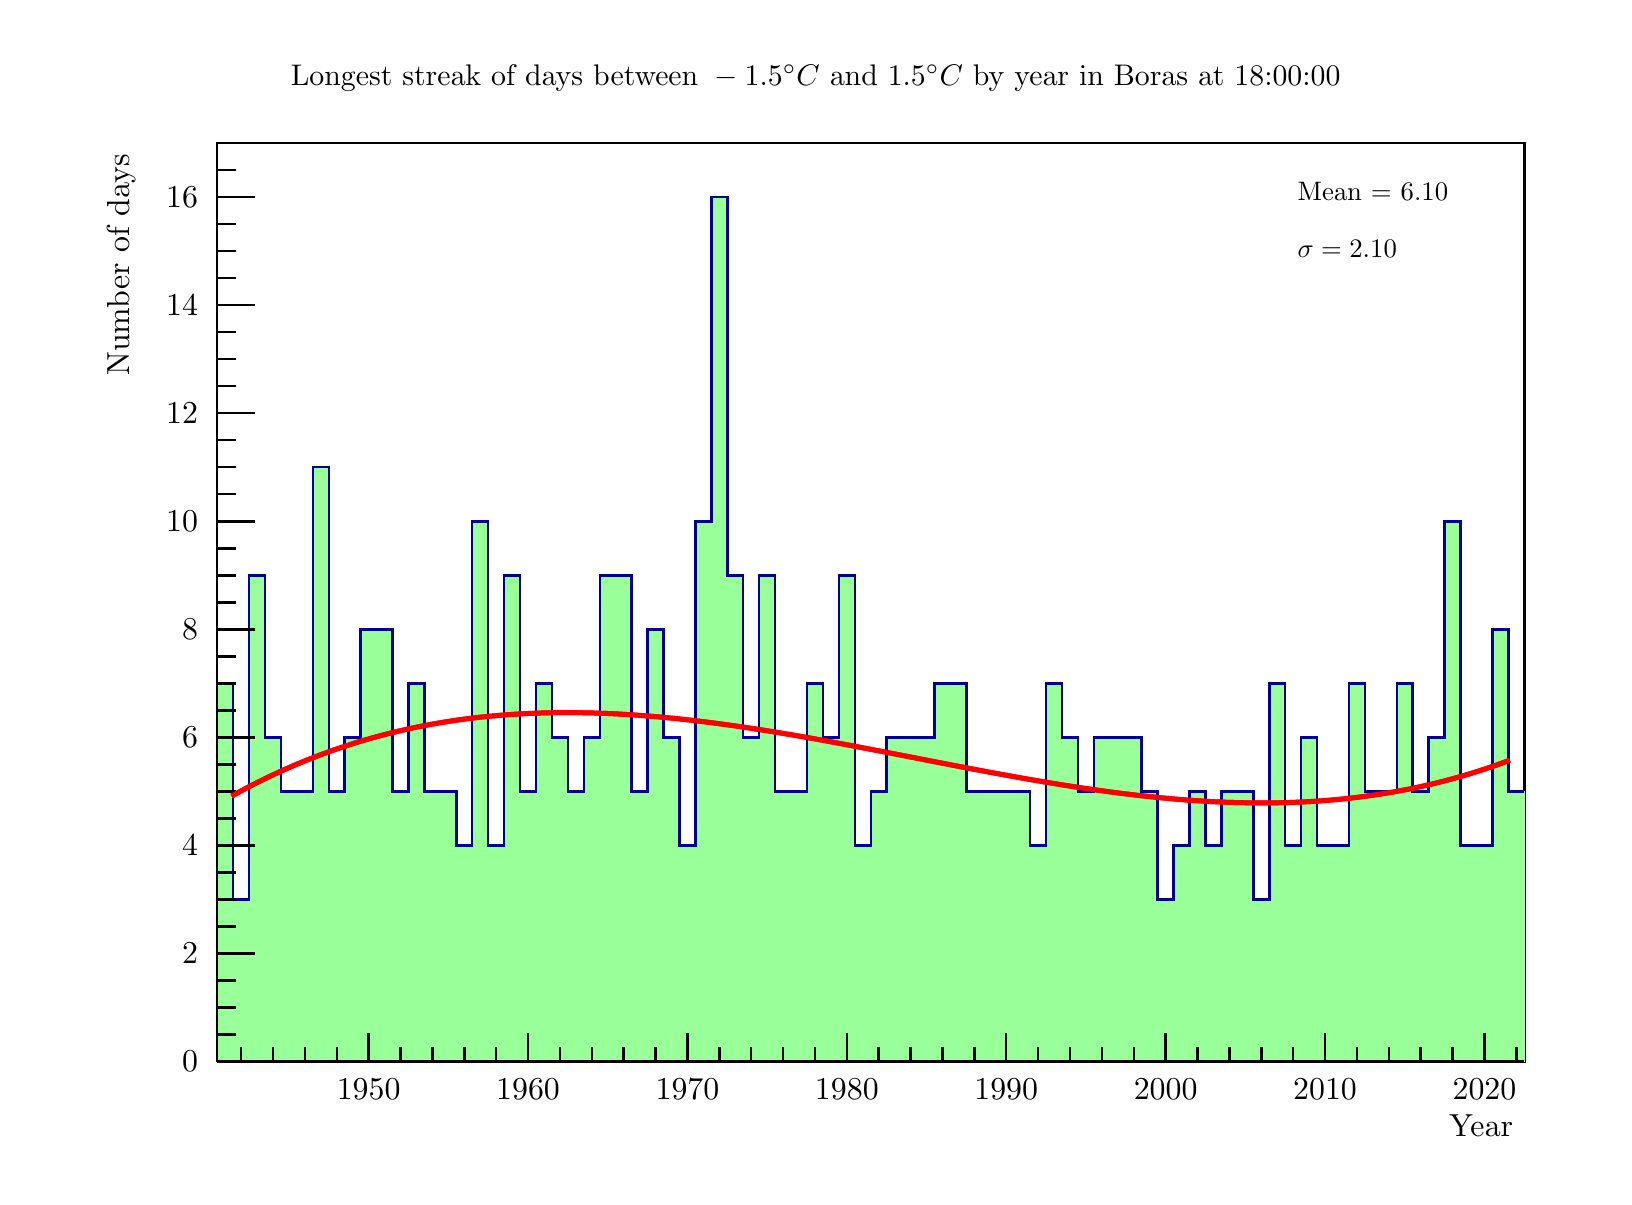
\begin{tikzpicture}
\def\CheckTikzLibraryLoaded#1{ \ifcsname tikz@library@#1@loaded\endcsname \else \PackageWarning{tikz}{usetikzlibrary{#1} is missing in the preamble.} \fi }
\CheckTikzLibraryLoaded{patterns}
\CheckTikzLibraryLoaded{plotmarks}
\pgfdeclareplotmark{cross} {
\pgfpathmoveto{\pgfpoint{-0.3\pgfplotmarksize}{\pgfplotmarksize}}
\pgfpathlineto{\pgfpoint{+0.3\pgfplotmarksize}{\pgfplotmarksize}}
\pgfpathlineto{\pgfpoint{+0.3\pgfplotmarksize}{0.3\pgfplotmarksize}}
\pgfpathlineto{\pgfpoint{+1\pgfplotmarksize}{0.3\pgfplotmarksize}}
\pgfpathlineto{\pgfpoint{+1\pgfplotmarksize}{-0.3\pgfplotmarksize}}
\pgfpathlineto{\pgfpoint{+0.3\pgfplotmarksize}{-0.3\pgfplotmarksize}}
\pgfpathlineto{\pgfpoint{+0.3\pgfplotmarksize}{-1.\pgfplotmarksize}}
\pgfpathlineto{\pgfpoint{-0.3\pgfplotmarksize}{-1.\pgfplotmarksize}}
\pgfpathlineto{\pgfpoint{-0.3\pgfplotmarksize}{-0.3\pgfplotmarksize}}
\pgfpathlineto{\pgfpoint{-1.\pgfplotmarksize}{-0.3\pgfplotmarksize}}
\pgfpathlineto{\pgfpoint{-1.\pgfplotmarksize}{0.3\pgfplotmarksize}}
\pgfpathlineto{\pgfpoint{-0.3\pgfplotmarksize}{0.3\pgfplotmarksize}}
\pgfpathclose
\pgfusepathqstroke
}
\pgfdeclareplotmark{cross*} {
\pgfpathmoveto{\pgfpoint{-0.3\pgfplotmarksize}{\pgfplotmarksize}}
\pgfpathlineto{\pgfpoint{+0.3\pgfplotmarksize}{\pgfplotmarksize}}
\pgfpathlineto{\pgfpoint{+0.3\pgfplotmarksize}{0.3\pgfplotmarksize}}
\pgfpathlineto{\pgfpoint{+1\pgfplotmarksize}{0.3\pgfplotmarksize}}
\pgfpathlineto{\pgfpoint{+1\pgfplotmarksize}{-0.3\pgfplotmarksize}}
\pgfpathlineto{\pgfpoint{+0.3\pgfplotmarksize}{-0.3\pgfplotmarksize}}
\pgfpathlineto{\pgfpoint{+0.3\pgfplotmarksize}{-1.\pgfplotmarksize}}
\pgfpathlineto{\pgfpoint{-0.3\pgfplotmarksize}{-1.\pgfplotmarksize}}
\pgfpathlineto{\pgfpoint{-0.3\pgfplotmarksize}{-0.3\pgfplotmarksize}}
\pgfpathlineto{\pgfpoint{-1.\pgfplotmarksize}{-0.3\pgfplotmarksize}}
\pgfpathlineto{\pgfpoint{-1.\pgfplotmarksize}{0.3\pgfplotmarksize}}
\pgfpathlineto{\pgfpoint{-0.3\pgfplotmarksize}{0.3\pgfplotmarksize}}
\pgfpathclose
\pgfusepathqfillstroke
}
\pgfdeclareplotmark{newstar} {
\pgfpathmoveto{\pgfqpoint{0pt}{\pgfplotmarksize}}
\pgfpathlineto{\pgfqpointpolar{44}{0.5\pgfplotmarksize}}
\pgfpathlineto{\pgfqpointpolar{18}{\pgfplotmarksize}}
\pgfpathlineto{\pgfqpointpolar{-20}{0.5\pgfplotmarksize}}
\pgfpathlineto{\pgfqpointpolar{-54}{\pgfplotmarksize}}
\pgfpathlineto{\pgfqpointpolar{-90}{0.5\pgfplotmarksize}}
\pgfpathlineto{\pgfqpointpolar{234}{\pgfplotmarksize}}
\pgfpathlineto{\pgfqpointpolar{198}{0.5\pgfplotmarksize}}
\pgfpathlineto{\pgfqpointpolar{162}{\pgfplotmarksize}}
\pgfpathlineto{\pgfqpointpolar{134}{0.5\pgfplotmarksize}}
\pgfpathclose
\pgfusepathqstroke
}
\pgfdeclareplotmark{newstar*} {
\pgfpathmoveto{\pgfqpoint{0pt}{\pgfplotmarksize}}
\pgfpathlineto{\pgfqpointpolar{44}{0.5\pgfplotmarksize}}
\pgfpathlineto{\pgfqpointpolar{18}{\pgfplotmarksize}}
\pgfpathlineto{\pgfqpointpolar{-20}{0.5\pgfplotmarksize}}
\pgfpathlineto{\pgfqpointpolar{-54}{\pgfplotmarksize}}
\pgfpathlineto{\pgfqpointpolar{-90}{0.5\pgfplotmarksize}}
\pgfpathlineto{\pgfqpointpolar{234}{\pgfplotmarksize}}
\pgfpathlineto{\pgfqpointpolar{198}{0.5\pgfplotmarksize}}
\pgfpathlineto{\pgfqpointpolar{162}{\pgfplotmarksize}}
\pgfpathlineto{\pgfqpointpolar{134}{0.5\pgfplotmarksize}}
\pgfpathclose
\pgfusepathqfillstroke
}
\definecolor{c}{rgb}{1,1,1};
\draw [color=c, fill=c] (0,0) rectangle (20,14.5819);
\draw [color=c, fill=c] (2.4,1.45819) rectangle (19,13.1237);
\definecolor{c}{rgb}{0,0,0};
\draw [c,line width=0.9] (2.4,1.45819) -- (2.4,13.1237) -- (19,13.1237) -- (19,1.45819) -- (2.4,1.45819);
\definecolor{c}{rgb}{1,1,1};
\draw [color=c, fill=c] (2.4,1.45819) rectangle (19,13.1237);
\definecolor{c}{rgb}{0,0,0};
\draw [c,line width=0.9] (2.4,1.45819) -- (2.4,13.1237) -- (19,13.1237) -- (19,1.45819) -- (2.4,1.45819);
\definecolor{c}{rgb}{0.6,1,0.6};
\draw [c, fill=c] (2.4,1.45819) -- (2.4,6.26166) -- (2.60244,6.26166) -- (2.60244,3.51682) -- (2.80488,3.51682) -- (2.80488,7.63407) -- (3.00732,7.63407) -- (3.00732,5.57545) -- (3.20976,5.57545) -- (3.20976,4.88924) -- (3.4122,4.88924) --
 (3.4122,4.88924) -- (3.61463,4.88924) -- (3.61463,9.00649) -- (3.81707,9.00649) -- (3.81707,4.88924) -- (4.01951,4.88924) -- (4.01951,5.57545) -- (4.22195,5.57545) -- (4.22195,6.94787) -- (4.42439,6.94787) -- (4.42439,6.94787) -- (4.62683,6.94787)
 -- (4.62683,4.88924) -- (4.82927,4.88924) -- (4.82927,6.26166) -- (5.03171,6.26166) -- (5.03171,4.88924) -- (5.23415,4.88924) -- (5.23415,4.88924) -- (5.43659,4.88924) -- (5.43659,4.20303) -- (5.63902,4.20303) -- (5.63902,8.32028) --
 (5.84146,8.32028) -- (5.84146,4.20303) -- (6.0439,4.20303) -- (6.0439,7.63407) -- (6.24634,7.63407) -- (6.24634,4.88924) -- (6.44878,4.88924) -- (6.44878,6.26166) -- (6.65122,6.26166) -- (6.65122,5.57545) -- (6.85366,5.57545) -- (6.85366,4.88924) --
 (7.0561,4.88924) -- (7.0561,5.57545) -- (7.25854,5.57545) -- (7.25854,7.63407) -- (7.46098,7.63407) -- (7.46098,7.63407) -- (7.66341,7.63407) -- (7.66341,4.88924) -- (7.86585,4.88924) -- (7.86585,6.94787) -- (8.06829,6.94787) -- (8.06829,5.57545) --
 (8.27073,5.57545) -- (8.27073,4.20303) -- (8.47317,4.20303) -- (8.47317,8.32028) -- (8.67561,8.32028) -- (8.67561,12.4375) -- (8.87805,12.4375) -- (8.87805,7.63407) -- (9.08049,7.63407) -- (9.08049,5.57545) -- (9.28293,5.57545) -- (9.28293,7.63407)
 -- (9.48537,7.63407) -- (9.48537,4.88924) -- (9.68781,4.88924) -- (9.68781,4.88924) -- (9.89024,4.88924) -- (9.89024,6.26166) -- (10.0927,6.26166) -- (10.0927,5.57545) -- (10.2951,5.57545) -- (10.2951,7.63407) -- (10.4976,7.63407) --
 (10.4976,4.20303) -- (10.7,4.20303) -- (10.7,4.88924) -- (10.9024,4.88924) -- (10.9024,5.57545) -- (11.1049,5.57545) -- (11.1049,5.57545) -- (11.3073,5.57545) -- (11.3073,5.57545) -- (11.5098,5.57545) -- (11.5098,6.26166) -- (11.7122,6.26166) --
 (11.7122,6.26166) -- (11.9146,6.26166) -- (11.9146,4.88924) -- (12.1171,4.88924) -- (12.1171,4.88924) -- (12.3195,4.88924) -- (12.3195,4.88924) -- (12.522,4.88924) -- (12.522,4.88924) -- (12.7244,4.88924) -- (12.7244,4.20303) -- (12.9268,4.20303) --
 (12.9268,6.26166) -- (13.1293,6.26166) -- (13.1293,5.57545) -- (13.3317,5.57545) -- (13.3317,4.88924) -- (13.5341,4.88924) -- (13.5341,5.57545) -- (13.7366,5.57545) -- (13.7366,5.57545) -- (13.939,5.57545) -- (13.939,5.57545) -- (14.1415,5.57545) --
 (14.1415,4.88924) -- (14.3439,4.88924) -- (14.3439,3.51682) -- (14.5463,3.51682) -- (14.5463,4.20303) -- (14.7488,4.20303) -- (14.7488,4.88924) -- (14.9512,4.88924) -- (14.9512,4.20303) -- (15.1537,4.20303) -- (15.1537,4.88924) -- (15.3561,4.88924)
 -- (15.3561,4.88924) -- (15.5585,4.88924) -- (15.5585,3.51682) -- (15.761,3.51682) -- (15.761,6.26166) -- (15.9634,6.26166) -- (15.9634,4.20303) -- (16.1659,4.20303) -- (16.1659,5.57545) -- (16.3683,5.57545) -- (16.3683,4.20303) -- (16.5707,4.20303)
 -- (16.5707,4.20303) -- (16.7732,4.20303) -- (16.7732,6.26166) -- (16.9756,6.26166) -- (16.9756,4.88924) -- (17.178,4.88924) -- (17.178,4.88924) -- (17.3805,4.88924) -- (17.3805,6.26166) -- (17.5829,6.26166) -- (17.5829,4.88924) -- (17.7854,4.88924)
 -- (17.7854,5.57545) -- (17.9878,5.57545) -- (17.9878,8.32028) -- (18.1902,8.32028) -- (18.1902,4.20303) -- (18.3927,4.20303) -- (18.3927,4.20303) -- (18.5951,4.20303) -- (18.5951,6.94787) -- (18.7976,6.94787) -- (18.7976,4.88924) -- (19,4.88924) --
 (19,1.45819);
\definecolor{c}{rgb}{0,0,0.6};
\draw [c,line width=0.9] (2.4,6.26166) -- (2.60244,6.26166) -- (2.60244,3.51682) -- (2.80488,3.51682) -- (2.80488,7.63407) -- (3.00732,7.63407) -- (3.00732,5.57545) -- (3.20976,5.57545) -- (3.20976,4.88924) -- (3.4122,4.88924) -- (3.4122,4.88924) --
 (3.61463,4.88924) -- (3.61463,9.00649) -- (3.81707,9.00649) -- (3.81707,4.88924) -- (4.01951,4.88924) -- (4.01951,5.57545) -- (4.22195,5.57545) -- (4.22195,6.94787) -- (4.42439,6.94787) -- (4.42439,6.94787) -- (4.62683,6.94787) -- (4.62683,4.88924)
 -- (4.82927,4.88924) -- (4.82927,6.26166) -- (5.03171,6.26166) -- (5.03171,4.88924) -- (5.23415,4.88924) -- (5.23415,4.88924) -- (5.43659,4.88924) -- (5.43659,4.20303) -- (5.63902,4.20303) -- (5.63902,8.32028) -- (5.84146,8.32028) --
 (5.84146,4.20303) -- (6.0439,4.20303) -- (6.0439,7.63407) -- (6.24634,7.63407) -- (6.24634,4.88924) -- (6.44878,4.88924) -- (6.44878,6.26166) -- (6.65122,6.26166) -- (6.65122,5.57545) -- (6.85366,5.57545) -- (6.85366,4.88924) -- (7.0561,4.88924) --
 (7.0561,5.57545) -- (7.25854,5.57545) -- (7.25854,7.63407) -- (7.46098,7.63407) -- (7.46098,7.63407) -- (7.66341,7.63407) -- (7.66341,4.88924) -- (7.86585,4.88924) -- (7.86585,6.94787) -- (8.06829,6.94787) -- (8.06829,5.57545) -- (8.27073,5.57545)
 -- (8.27073,4.20303) -- (8.47317,4.20303) -- (8.47317,8.32028) -- (8.67561,8.32028) -- (8.67561,12.4375) -- (8.87805,12.4375) -- (8.87805,7.63407) -- (9.08049,7.63407) -- (9.08049,5.57545) -- (9.28293,5.57545) -- (9.28293,7.63407) --
 (9.48537,7.63407) -- (9.48537,4.88924) -- (9.68781,4.88924) -- (9.68781,4.88924) -- (9.89024,4.88924) -- (9.89024,6.26166) -- (10.0927,6.26166) -- (10.0927,5.57545) -- (10.2951,5.57545) -- (10.2951,7.63407) -- (10.4976,7.63407) -- (10.4976,4.20303)
 -- (10.7,4.20303) -- (10.7,4.88924) -- (10.9024,4.88924) -- (10.9024,5.57545) -- (11.1049,5.57545) -- (11.1049,5.57545) -- (11.3073,5.57545) -- (11.3073,5.57545) -- (11.5098,5.57545) -- (11.5098,6.26166) -- (11.7122,6.26166) -- (11.7122,6.26166) --
 (11.9146,6.26166) -- (11.9146,4.88924) -- (12.1171,4.88924) -- (12.1171,4.88924) -- (12.3195,4.88924) -- (12.3195,4.88924) -- (12.522,4.88924) -- (12.522,4.88924) -- (12.7244,4.88924) -- (12.7244,4.20303) -- (12.9268,4.20303) -- (12.9268,6.26166) --
 (13.1293,6.26166) -- (13.1293,5.57545) -- (13.3317,5.57545) -- (13.3317,4.88924) -- (13.5341,4.88924) -- (13.5341,5.57545) -- (13.7366,5.57545) -- (13.7366,5.57545) -- (13.939,5.57545) -- (13.939,5.57545) -- (14.1415,5.57545) -- (14.1415,4.88924) --
 (14.3439,4.88924) -- (14.3439,3.51682) -- (14.5463,3.51682) -- (14.5463,4.20303) -- (14.7488,4.20303) -- (14.7488,4.88924) -- (14.9512,4.88924) -- (14.9512,4.20303) -- (15.1537,4.20303) -- (15.1537,4.88924) -- (15.3561,4.88924) -- (15.3561,4.88924)
 -- (15.5585,4.88924) -- (15.5585,3.51682) -- (15.761,3.51682) -- (15.761,6.26166) -- (15.9634,6.26166) -- (15.9634,4.20303) -- (16.1659,4.20303) -- (16.1659,5.57545) -- (16.3683,5.57545) -- (16.3683,4.20303) -- (16.5707,4.20303) -- (16.5707,4.20303)
 -- (16.7732,4.20303) -- (16.7732,6.26166) -- (16.9756,6.26166) -- (16.9756,4.88924) -- (17.178,4.88924) -- (17.178,4.88924) -- (17.3805,4.88924) -- (17.3805,6.26166) -- (17.5829,6.26166) -- (17.5829,4.88924) -- (17.7854,4.88924) -- (17.7854,5.57545)
 -- (17.9878,5.57545) -- (17.9878,8.32028) -- (18.1902,8.32028) -- (18.1902,4.20303) -- (18.3927,4.20303) -- (18.3927,4.20303) -- (18.5951,4.20303) -- (18.5951,6.94787) -- (18.7976,6.94787) -- (18.7976,4.88924) -- (19,4.88924);
\definecolor{c}{rgb}{1,0,0};
\draw [c,line width=1.8] (2.58321,4.82977) -- (2.74718,4.91903) -- (2.91116,5.00371) -- (3.07513,5.08389) -- (3.23911,5.15966) -- (3.40309,5.23112) -- (3.56706,5.29834) -- (3.73104,5.36142) -- (3.89501,5.42045) -- (4.05899,5.4755) --
 (4.22296,5.52669) -- (4.38694,5.57408) -- (4.55091,5.61777) -- (4.71489,5.65785) -- (4.87887,5.6944) -- (5.04284,5.72751) -- (5.20682,5.75728) -- (5.37079,5.78379) -- (5.53477,5.80713) -- (5.69874,5.82739) -- (5.86272,5.84465) -- (6.0267,5.85901) --
 (6.19067,5.87055) -- (6.35465,5.87936) -- (6.51862,5.88553) -- (6.6826,5.88914) -- (6.84657,5.89029) -- (7.01055,5.88907) -- (7.17452,5.88556) -- (7.3385,5.87985) -- (7.50248,5.87203) -- (7.66645,5.86219) -- (7.83043,5.85041) -- (7.9944,5.83679) --
 (8.15838,5.82141) -- (8.32235,5.80437) -- (8.48633,5.78574) -- (8.6503,5.76562) -- (8.81428,5.7441) -- (8.97826,5.72126) -- (9.14223,5.6972) -- (9.30621,5.67199) -- (9.47018,5.64574) -- (9.63416,5.61852) -- (9.79813,5.59043) -- (9.96211,5.56156) --
 (10.1261,5.53199) -- (10.2901,5.50181) -- (10.454,5.47111) -- (10.618,5.43998);
\draw [c,line width=1.8] (10.618,5.43998) -- (10.782,5.40851) -- (10.946,5.37678) -- (11.1099,5.34489) -- (11.2739,5.31291) -- (11.4379,5.28095) -- (11.6019,5.24909) -- (11.7658,5.21741) -- (11.9298,5.18601) -- (12.0938,5.15497) -- (12.2578,5.12439)
 -- (12.4217,5.09434) -- (12.5857,5.06492) -- (12.7497,5.03623) -- (12.9137,5.00833) -- (13.0776,4.98133) -- (13.2416,4.95532) -- (13.4056,4.93037) -- (13.5696,4.90658) -- (13.7335,4.88404) -- (13.8975,4.86284) -- (14.0615,4.84306) --
 (14.2255,4.82479) -- (14.3895,4.80812) -- (14.5534,4.79315) -- (14.7174,4.77995) -- (14.8814,4.76861) -- (15.0454,4.75923) -- (15.2093,4.7519) -- (15.3733,4.74669) -- (15.5373,4.74371) -- (15.7013,4.74303) -- (15.8652,4.74475) -- (16.0292,4.74895)
 -- (16.1932,4.75572) -- (16.3572,4.76516) -- (16.5211,4.77735) -- (16.6851,4.79237) -- (16.8491,4.81032) -- (17.0131,4.83129) -- (17.177,4.85536) -- (17.341,4.88262) -- (17.505,4.91316) -- (17.669,4.94707) -- (17.8329,4.98443) -- (17.9969,5.02534)
 -- (18.1609,5.06989) -- (18.3249,5.11815) -- (18.4888,5.17023) -- (18.6528,5.2262);
\draw [c,line width=1.8] (18.6528,5.2262) -- (18.8168,5.28616);
\definecolor{c}{rgb}{0,0,0};
\draw [c,line width=0.9] (2.4,1.45819) -- (19,1.45819);
\draw [c,line width=0.9] (4.32317,1.82128) -- (4.32317,1.45819);
\draw [c,line width=0.9] (4.72805,1.63974) -- (4.72805,1.45819);
\draw [c,line width=0.9] (5.13293,1.63974) -- (5.13293,1.45819);
\draw [c,line width=0.9] (5.53781,1.63974) -- (5.53781,1.45819);
\draw [c,line width=0.9] (5.94268,1.63974) -- (5.94268,1.45819);
\draw [c,line width=0.9] (6.34756,1.82128) -- (6.34756,1.45819);
\draw [c,line width=0.9] (6.75244,1.63974) -- (6.75244,1.45819);
\draw [c,line width=0.9] (7.15732,1.63974) -- (7.15732,1.45819);
\draw [c,line width=0.9] (7.5622,1.63974) -- (7.5622,1.45819);
\draw [c,line width=0.9] (7.96707,1.63974) -- (7.96707,1.45819);
\draw [c,line width=0.9] (8.37195,1.82128) -- (8.37195,1.45819);
\draw [c,line width=0.9] (8.77683,1.63974) -- (8.77683,1.45819);
\draw [c,line width=0.9] (9.18171,1.63974) -- (9.18171,1.45819);
\draw [c,line width=0.9] (9.58659,1.63974) -- (9.58659,1.45819);
\draw [c,line width=0.9] (9.99146,1.63974) -- (9.99146,1.45819);
\draw [c,line width=0.9] (10.3963,1.82128) -- (10.3963,1.45819);
\draw [c,line width=0.9] (10.8012,1.63974) -- (10.8012,1.45819);
\draw [c,line width=0.9] (11.2061,1.63974) -- (11.2061,1.45819);
\draw [c,line width=0.9] (11.611,1.63974) -- (11.611,1.45819);
\draw [c,line width=0.9] (12.0159,1.63974) -- (12.0159,1.45819);
\draw [c,line width=0.9] (12.4207,1.82128) -- (12.4207,1.45819);
\draw [c,line width=0.9] (12.8256,1.63974) -- (12.8256,1.45819);
\draw [c,line width=0.9] (13.2305,1.63974) -- (13.2305,1.45819);
\draw [c,line width=0.9] (13.6354,1.63974) -- (13.6354,1.45819);
\draw [c,line width=0.9] (14.0402,1.63974) -- (14.0402,1.45819);
\draw [c,line width=0.9] (14.4451,1.82128) -- (14.4451,1.45819);
\draw [c,line width=0.9] (14.85,1.63974) -- (14.85,1.45819);
\draw [c,line width=0.9] (15.2549,1.63974) -- (15.2549,1.45819);
\draw [c,line width=0.9] (15.6598,1.63974) -- (15.6598,1.45819);
\draw [c,line width=0.9] (16.0646,1.63974) -- (16.0646,1.45819);
\draw [c,line width=0.9] (16.4695,1.82128) -- (16.4695,1.45819);
\draw [c,line width=0.9] (16.8744,1.63974) -- (16.8744,1.45819);
\draw [c,line width=0.9] (17.2793,1.63974) -- (17.2793,1.45819);
\draw [c,line width=0.9] (17.6841,1.63974) -- (17.6841,1.45819);
\draw [c,line width=0.9] (18.089,1.63974) -- (18.089,1.45819);
\draw [c,line width=0.9] (18.4939,1.82128) -- (18.4939,1.45819);
\draw [c,line width=0.9] (4.32317,1.82128) -- (4.32317,1.45819);
\draw [c,line width=0.9] (3.91829,1.63974) -- (3.91829,1.45819);
\draw [c,line width=0.9] (3.51341,1.63974) -- (3.51341,1.45819);
\draw [c,line width=0.9] (3.10854,1.63974) -- (3.10854,1.45819);
\draw [c,line width=0.9] (2.70366,1.63974) -- (2.70366,1.45819);
\draw [c,line width=0.9] (18.4939,1.82128) -- (18.4939,1.45819);
\draw [c,line width=0.9] (18.8988,1.63974) -- (18.8988,1.45819);
\draw [anchor=base] (4.32317,0.97699) node[scale=1.15134, color=c, rotate=0]{1950};
\draw [anchor=base] (6.34756,0.97699) node[scale=1.15134, color=c, rotate=0]{1960};
\draw [anchor=base] (8.37195,0.97699) node[scale=1.15134, color=c, rotate=0]{1970};
\draw [anchor=base] (10.3963,0.97699) node[scale=1.15134, color=c, rotate=0]{1980};
\draw [anchor=base] (12.4207,0.97699) node[scale=1.15134, color=c, rotate=0]{1990};
\draw [anchor=base] (14.4451,0.97699) node[scale=1.15134, color=c, rotate=0]{2000};
\draw [anchor=base] (16.4695,0.97699) node[scale=1.15134, color=c, rotate=0]{2010};
\draw [anchor=base] (18.4939,0.97699) node[scale=1.15134, color=c, rotate=0]{2020};
\draw [anchor= east] (19,0.641605) node[scale=1.15134, color=c, rotate=0]{Year};
\draw [c,line width=0.9] (2.4,1.45819) -- (2.4,13.1237);
\draw [c,line width=0.9] (2.88,1.45819) -- (2.4,1.45819);
\draw [c,line width=0.9] (2.64,1.8013) -- (2.4,1.8013);
\draw [c,line width=0.9] (2.64,2.1444) -- (2.4,2.1444);
\draw [c,line width=0.9] (2.64,2.48751) -- (2.4,2.48751);
\draw [c,line width=0.9] (2.88,2.83061) -- (2.4,2.83061);
\draw [c,line width=0.9] (2.64,3.17372) -- (2.4,3.17372);
\draw [c,line width=0.9] (2.64,3.51682) -- (2.4,3.51682);
\draw [c,line width=0.9] (2.64,3.85993) -- (2.4,3.85993);
\draw [c,line width=0.9] (2.88,4.20303) -- (2.4,4.20303);
\draw [c,line width=0.9] (2.64,4.54613) -- (2.4,4.54613);
\draw [c,line width=0.9] (2.64,4.88924) -- (2.4,4.88924);
\draw [c,line width=0.9] (2.64,5.23234) -- (2.4,5.23234);
\draw [c,line width=0.9] (2.88,5.57545) -- (2.4,5.57545);
\draw [c,line width=0.9] (2.64,5.91855) -- (2.4,5.91855);
\draw [c,line width=0.9] (2.64,6.26166) -- (2.4,6.26166);
\draw [c,line width=0.9] (2.64,6.60476) -- (2.4,6.60476);
\draw [c,line width=0.9] (2.88,6.94787) -- (2.4,6.94787);
\draw [c,line width=0.9] (2.64,7.29097) -- (2.4,7.29097);
\draw [c,line width=0.9] (2.64,7.63407) -- (2.4,7.63407);
\draw [c,line width=0.9] (2.64,7.97718) -- (2.4,7.97718);
\draw [c,line width=0.9] (2.88,8.32028) -- (2.4,8.32028);
\draw [c,line width=0.9] (2.64,8.66339) -- (2.4,8.66339);
\draw [c,line width=0.9] (2.64,9.00649) -- (2.4,9.00649);
\draw [c,line width=0.9] (2.64,9.3496) -- (2.4,9.3496);
\draw [c,line width=0.9] (2.88,9.6927) -- (2.4,9.6927);
\draw [c,line width=0.9] (2.64,10.0358) -- (2.4,10.0358);
\draw [c,line width=0.9] (2.64,10.3789) -- (2.4,10.3789);
\draw [c,line width=0.9] (2.64,10.722) -- (2.4,10.722);
\draw [c,line width=0.9] (2.88,11.0651) -- (2.4,11.0651);
\draw [c,line width=0.9] (2.64,11.4082) -- (2.4,11.4082);
\draw [c,line width=0.9] (2.64,11.7513) -- (2.4,11.7513);
\draw [c,line width=0.9] (2.64,12.0944) -- (2.4,12.0944);
\draw [c,line width=0.9] (2.88,12.4375) -- (2.4,12.4375);
\draw [c,line width=0.9] (2.88,12.4375) -- (2.4,12.4375);
\draw [c,line width=0.9] (2.64,12.7806) -- (2.4,12.7806);
\draw [c,line width=0.9] (2.64,13.1237) -- (2.4,13.1237);
\draw [anchor= east] (2.3,1.45819) node[scale=1.15134, color=c, rotate=0]{0};
\draw [anchor= east] (2.3,2.83061) node[scale=1.15134, color=c, rotate=0]{2};
\draw [anchor= east] (2.3,4.20303) node[scale=1.15134, color=c, rotate=0]{4};
\draw [anchor= east] (2.3,5.57545) node[scale=1.15134, color=c, rotate=0]{6};
\draw [anchor= east] (2.3,6.94787) node[scale=1.15134, color=c, rotate=0]{8};
\draw [anchor= east] (2.3,8.32028) node[scale=1.15134, color=c, rotate=0]{10};
\draw [anchor= east] (2.3,9.6927) node[scale=1.15134, color=c, rotate=0]{12};
\draw [anchor= east] (2.3,11.0651) node[scale=1.15134, color=c, rotate=0]{14};
\draw [anchor= east] (2.3,12.4375) node[scale=1.15134, color=c, rotate=0]{16};
\draw [anchor= east] (1.18161,13.1237) node[scale=1.15134, color=c, rotate=90]{Number of days};
\definecolor{c}{rgb}{1,0,0};
\draw [c,line width=1.8] (2.58321,4.82977) -- (2.74718,4.91903) -- (2.91116,5.00371) -- (3.07513,5.08389) -- (3.23911,5.15966) -- (3.40309,5.23112) -- (3.56706,5.29834) -- (3.73104,5.36142) -- (3.89501,5.42045) -- (4.05899,5.4755) --
 (4.22296,5.52669) -- (4.38694,5.57408) -- (4.55091,5.61777) -- (4.71489,5.65785) -- (4.87887,5.6944) -- (5.04284,5.72751) -- (5.20682,5.75728) -- (5.37079,5.78379) -- (5.53477,5.80713) -- (5.69874,5.82739) -- (5.86272,5.84465) -- (6.0267,5.85901) --
 (6.19067,5.87055) -- (6.35465,5.87936) -- (6.51862,5.88553) -- (6.6826,5.88914) -- (6.84657,5.89029) -- (7.01055,5.88907) -- (7.17452,5.88556) -- (7.3385,5.87985) -- (7.50248,5.87203) -- (7.66645,5.86219) -- (7.83043,5.85041) -- (7.9944,5.83679) --
 (8.15838,5.82141) -- (8.32235,5.80437) -- (8.48633,5.78574) -- (8.6503,5.76562) -- (8.81428,5.7441) -- (8.97826,5.72126) -- (9.14223,5.6972) -- (9.30621,5.67199) -- (9.47018,5.64574) -- (9.63416,5.61852) -- (9.79813,5.59043) -- (9.96211,5.56156) --
 (10.1261,5.53199) -- (10.2901,5.50181) -- (10.454,5.47111) -- (10.618,5.43998);
\draw [c,line width=1.8] (10.618,5.43998) -- (10.782,5.40851) -- (10.946,5.37678) -- (11.1099,5.34489) -- (11.2739,5.31291) -- (11.4379,5.28095) -- (11.6019,5.24909) -- (11.7658,5.21741) -- (11.9298,5.18601) -- (12.0938,5.15497) -- (12.2578,5.12439)
 -- (12.4217,5.09434) -- (12.5857,5.06492) -- (12.7497,5.03623) -- (12.9137,5.00833) -- (13.0776,4.98133) -- (13.2416,4.95532) -- (13.4056,4.93037) -- (13.5696,4.90658) -- (13.7335,4.88404) -- (13.8975,4.86284) -- (14.0615,4.84306) --
 (14.2255,4.82479) -- (14.3895,4.80812) -- (14.5534,4.79315) -- (14.7174,4.77995) -- (14.8814,4.76861) -- (15.0454,4.75923) -- (15.2093,4.7519) -- (15.3733,4.74669) -- (15.5373,4.74371) -- (15.7013,4.74303) -- (15.8652,4.74475) -- (16.0292,4.74895)
 -- (16.1932,4.75572) -- (16.3572,4.76516) -- (16.5211,4.77735) -- (16.6851,4.79237) -- (16.8491,4.81032) -- (17.0131,4.83129) -- (17.177,4.85536) -- (17.341,4.88262) -- (17.505,4.91316) -- (17.669,4.94707) -- (17.8329,4.98443) -- (17.9969,5.02534)
 -- (18.1609,5.06989) -- (18.3249,5.11815) -- (18.4888,5.17023) -- (18.6528,5.2262);
\draw [c,line width=1.8] (18.6528,5.2262) -- (18.8168,5.28616);
\definecolor{c}{rgb}{0,0,0};
\draw [anchor=base west] (16,12.3946) node[scale=0.965639, color=c, rotate=0]{Mean = 6.10};
\draw [anchor=base west] (16,11.6656) node[scale=0.965639, color=c, rotate=0]{$\sigma = 2.10$};
\draw (10,13.9476) node[scale=1.07706, color=c, rotate=0]{$\text{Longest streak of days between }-1.5^{\circ}C\text{ and }1.5^{\circ}C\text{ by year in }\text{Boras at 18:00:00}$};
\end{tikzpicture}
%\end{document}
}
    \label{fig:enter-label}
\end{figure}

Similarly, in Visby, 1972 saw a long 17-day streak of around $0^\circ C$ at 12:00:00. 

\begin{figure}[H]
    \centering
    \scalebox{.5}{%\documentclass{standalone}
%\usepackage{tikz}
%\usetikzlibrary{patterns,plotmarks}
%\begin{document}
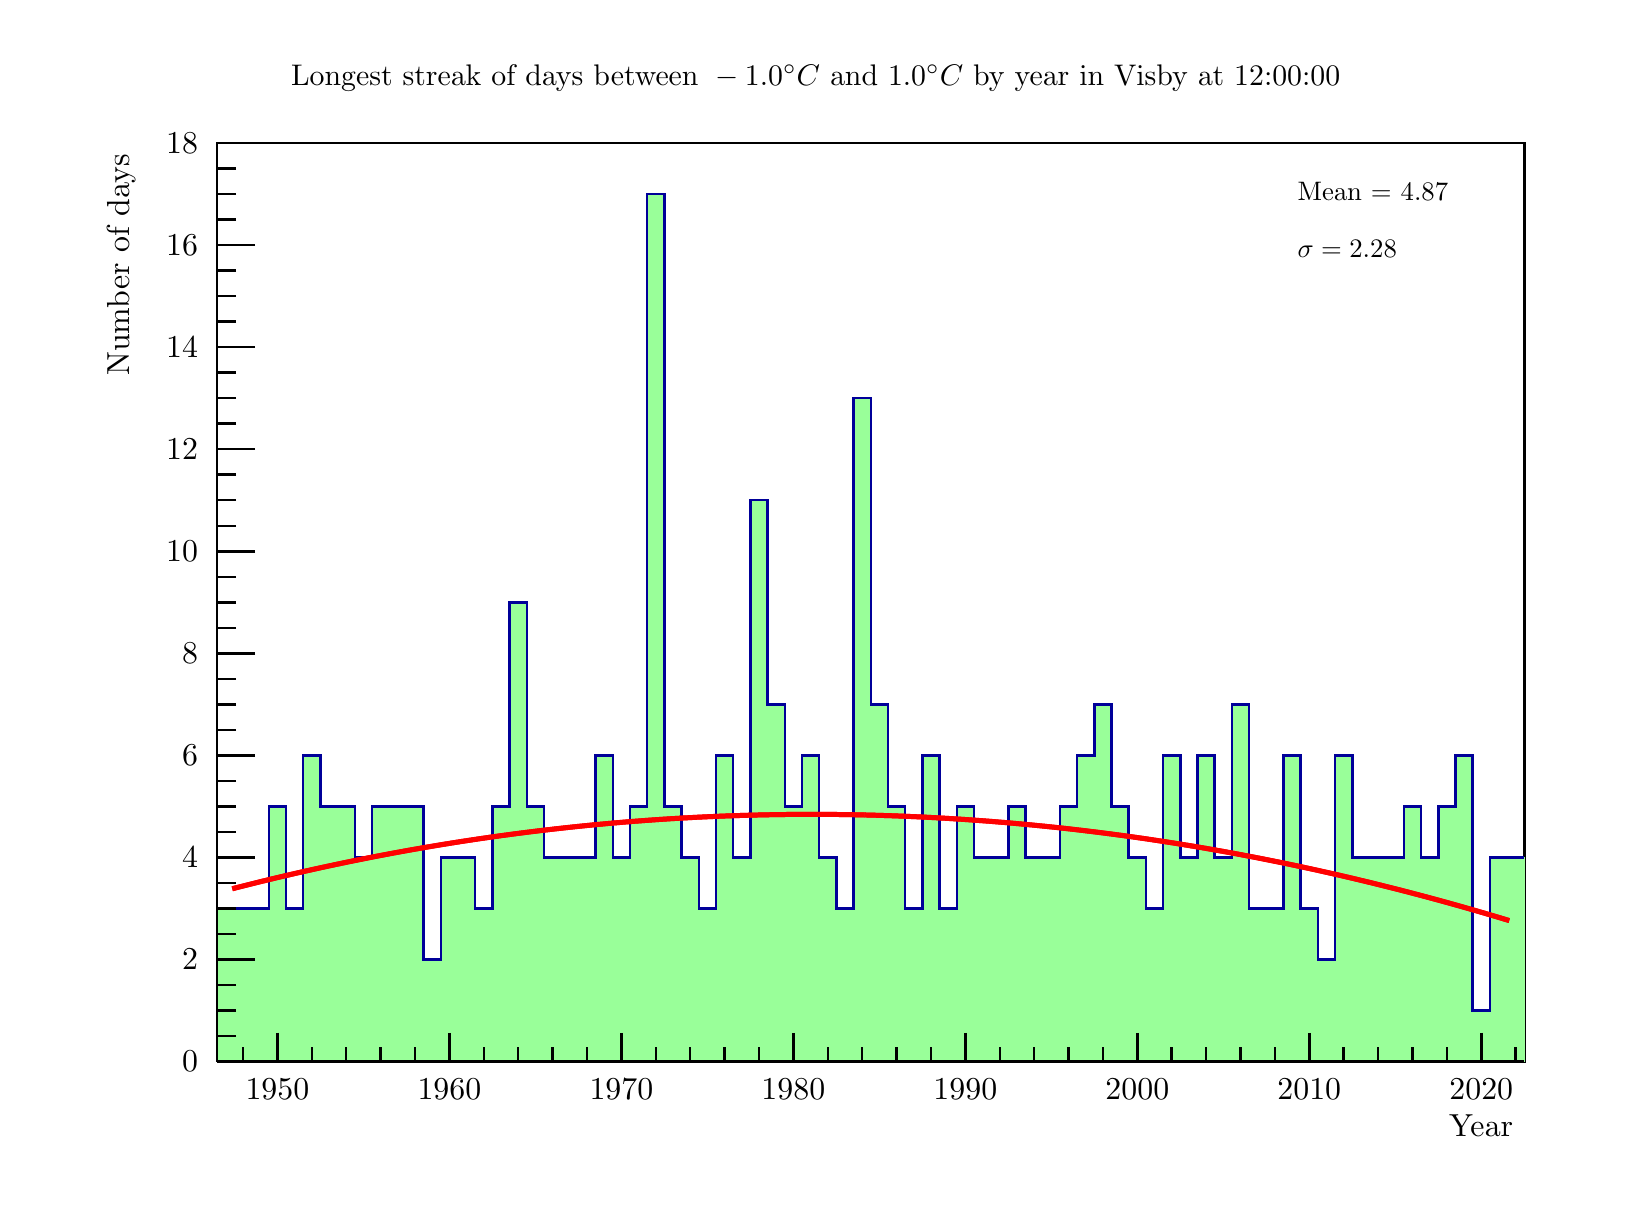
\begin{tikzpicture}
\def\CheckTikzLibraryLoaded#1{ \ifcsname tikz@library@#1@loaded\endcsname \else \PackageWarning{tikz}{usetikzlibrary{#1} is missing in the preamble.} \fi }
\CheckTikzLibraryLoaded{patterns}
\CheckTikzLibraryLoaded{plotmarks}
\pgfdeclareplotmark{cross} {
\pgfpathmoveto{\pgfpoint{-0.3\pgfplotmarksize}{\pgfplotmarksize}}
\pgfpathlineto{\pgfpoint{+0.3\pgfplotmarksize}{\pgfplotmarksize}}
\pgfpathlineto{\pgfpoint{+0.3\pgfplotmarksize}{0.3\pgfplotmarksize}}
\pgfpathlineto{\pgfpoint{+1\pgfplotmarksize}{0.3\pgfplotmarksize}}
\pgfpathlineto{\pgfpoint{+1\pgfplotmarksize}{-0.3\pgfplotmarksize}}
\pgfpathlineto{\pgfpoint{+0.3\pgfplotmarksize}{-0.3\pgfplotmarksize}}
\pgfpathlineto{\pgfpoint{+0.3\pgfplotmarksize}{-1.\pgfplotmarksize}}
\pgfpathlineto{\pgfpoint{-0.3\pgfplotmarksize}{-1.\pgfplotmarksize}}
\pgfpathlineto{\pgfpoint{-0.3\pgfplotmarksize}{-0.3\pgfplotmarksize}}
\pgfpathlineto{\pgfpoint{-1.\pgfplotmarksize}{-0.3\pgfplotmarksize}}
\pgfpathlineto{\pgfpoint{-1.\pgfplotmarksize}{0.3\pgfplotmarksize}}
\pgfpathlineto{\pgfpoint{-0.3\pgfplotmarksize}{0.3\pgfplotmarksize}}
\pgfpathclose
\pgfusepathqstroke
}
\pgfdeclareplotmark{cross*} {
\pgfpathmoveto{\pgfpoint{-0.3\pgfplotmarksize}{\pgfplotmarksize}}
\pgfpathlineto{\pgfpoint{+0.3\pgfplotmarksize}{\pgfplotmarksize}}
\pgfpathlineto{\pgfpoint{+0.3\pgfplotmarksize}{0.3\pgfplotmarksize}}
\pgfpathlineto{\pgfpoint{+1\pgfplotmarksize}{0.3\pgfplotmarksize}}
\pgfpathlineto{\pgfpoint{+1\pgfplotmarksize}{-0.3\pgfplotmarksize}}
\pgfpathlineto{\pgfpoint{+0.3\pgfplotmarksize}{-0.3\pgfplotmarksize}}
\pgfpathlineto{\pgfpoint{+0.3\pgfplotmarksize}{-1.\pgfplotmarksize}}
\pgfpathlineto{\pgfpoint{-0.3\pgfplotmarksize}{-1.\pgfplotmarksize}}
\pgfpathlineto{\pgfpoint{-0.3\pgfplotmarksize}{-0.3\pgfplotmarksize}}
\pgfpathlineto{\pgfpoint{-1.\pgfplotmarksize}{-0.3\pgfplotmarksize}}
\pgfpathlineto{\pgfpoint{-1.\pgfplotmarksize}{0.3\pgfplotmarksize}}
\pgfpathlineto{\pgfpoint{-0.3\pgfplotmarksize}{0.3\pgfplotmarksize}}
\pgfpathclose
\pgfusepathqfillstroke
}
\pgfdeclareplotmark{newstar} {
\pgfpathmoveto{\pgfqpoint{0pt}{\pgfplotmarksize}}
\pgfpathlineto{\pgfqpointpolar{44}{0.5\pgfplotmarksize}}
\pgfpathlineto{\pgfqpointpolar{18}{\pgfplotmarksize}}
\pgfpathlineto{\pgfqpointpolar{-20}{0.5\pgfplotmarksize}}
\pgfpathlineto{\pgfqpointpolar{-54}{\pgfplotmarksize}}
\pgfpathlineto{\pgfqpointpolar{-90}{0.5\pgfplotmarksize}}
\pgfpathlineto{\pgfqpointpolar{234}{\pgfplotmarksize}}
\pgfpathlineto{\pgfqpointpolar{198}{0.5\pgfplotmarksize}}
\pgfpathlineto{\pgfqpointpolar{162}{\pgfplotmarksize}}
\pgfpathlineto{\pgfqpointpolar{134}{0.5\pgfplotmarksize}}
\pgfpathclose
\pgfusepathqstroke
}
\pgfdeclareplotmark{newstar*} {
\pgfpathmoveto{\pgfqpoint{0pt}{\pgfplotmarksize}}
\pgfpathlineto{\pgfqpointpolar{44}{0.5\pgfplotmarksize}}
\pgfpathlineto{\pgfqpointpolar{18}{\pgfplotmarksize}}
\pgfpathlineto{\pgfqpointpolar{-20}{0.5\pgfplotmarksize}}
\pgfpathlineto{\pgfqpointpolar{-54}{\pgfplotmarksize}}
\pgfpathlineto{\pgfqpointpolar{-90}{0.5\pgfplotmarksize}}
\pgfpathlineto{\pgfqpointpolar{234}{\pgfplotmarksize}}
\pgfpathlineto{\pgfqpointpolar{198}{0.5\pgfplotmarksize}}
\pgfpathlineto{\pgfqpointpolar{162}{\pgfplotmarksize}}
\pgfpathlineto{\pgfqpointpolar{134}{0.5\pgfplotmarksize}}
\pgfpathclose
\pgfusepathqfillstroke
}
\definecolor{c}{rgb}{1,1,1};
\draw [color=c, fill=c] (0,0) rectangle (20,14.5819);
\draw [color=c, fill=c] (2.4,1.45819) rectangle (19,13.1237);
\definecolor{c}{rgb}{0,0,0};
\draw [c,line width=0.9] (2.4,1.45819) -- (2.4,13.1237) -- (19,13.1237) -- (19,1.45819) -- (2.4,1.45819);
\definecolor{c}{rgb}{1,1,1};
\draw [color=c, fill=c] (2.4,1.45819) rectangle (19,13.1237);
\definecolor{c}{rgb}{0,0,0};
\draw [c,line width=0.9] (2.4,1.45819) -- (2.4,13.1237) -- (19,13.1237) -- (19,1.45819) -- (2.4,1.45819);
\definecolor{c}{rgb}{0.6,1,0.6};
\draw [c, fill=c] (2.4,1.45819) -- (2.4,3.40245) -- (2.61842,3.40245) -- (2.61842,3.40245) -- (2.83684,3.40245) -- (2.83684,3.40245) -- (3.05526,3.40245) -- (3.05526,4.69863) -- (3.27368,4.69863) -- (3.27368,3.40245) -- (3.49211,3.40245) --
 (3.49211,5.34671) -- (3.71053,5.34671) -- (3.71053,4.69863) -- (3.92895,4.69863) -- (3.92895,4.69863) -- (4.14737,4.69863) -- (4.14737,4.05054) -- (4.36579,4.05054) -- (4.36579,4.69863) -- (4.58421,4.69863) -- (4.58421,4.69863) -- (4.80263,4.69863)
 -- (4.80263,4.69863) -- (5.02105,4.69863) -- (5.02105,2.75437) -- (5.23947,2.75437) -- (5.23947,4.05054) -- (5.45789,4.05054) -- (5.45789,4.05054) -- (5.67632,4.05054) -- (5.67632,3.40245) -- (5.89474,3.40245) -- (5.89474,4.69863) --
 (6.11316,4.69863) -- (6.11316,7.29097) -- (6.33158,7.29097) -- (6.33158,4.69863) -- (6.55,4.69863) -- (6.55,4.05054) -- (6.76842,4.05054) -- (6.76842,4.05054) -- (6.98684,4.05054) -- (6.98684,4.05054) -- (7.20526,4.05054) -- (7.20526,5.34671) --
 (7.42368,5.34671) -- (7.42368,4.05054) -- (7.64211,4.05054) -- (7.64211,4.69863) -- (7.86053,4.69863) -- (7.86053,12.4757) -- (8.07895,12.4757) -- (8.07895,4.69863) -- (8.29737,4.69863) -- (8.29737,4.05054) -- (8.51579,4.05054) -- (8.51579,3.40245)
 -- (8.73421,3.40245) -- (8.73421,5.34671) -- (8.95263,5.34671) -- (8.95263,4.05054) -- (9.17105,4.05054) -- (9.17105,8.58714) -- (9.38947,8.58714) -- (9.38947,5.9948) -- (9.60789,5.9948) -- (9.60789,4.69863) -- (9.82632,4.69863) -- (9.82632,5.34671)
 -- (10.0447,5.34671) -- (10.0447,4.05054) -- (10.2632,4.05054) -- (10.2632,3.40245) -- (10.4816,3.40245) -- (10.4816,9.88332) -- (10.7,9.88332) -- (10.7,5.9948) -- (10.9184,5.9948) -- (10.9184,4.69863) -- (11.1368,4.69863) -- (11.1368,3.40245) --
 (11.3553,3.40245) -- (11.3553,5.34671) -- (11.5737,5.34671) -- (11.5737,3.40245) -- (11.7921,3.40245) -- (11.7921,4.69863) -- (12.0105,4.69863) -- (12.0105,4.05054) -- (12.2289,4.05054) -- (12.2289,4.05054) -- (12.4474,4.05054) -- (12.4474,4.69863)
 -- (12.6658,4.69863) -- (12.6658,4.05054) -- (12.8842,4.05054) -- (12.8842,4.05054) -- (13.1026,4.05054) -- (13.1026,4.69863) -- (13.3211,4.69863) -- (13.3211,5.34671) -- (13.5395,5.34671) -- (13.5395,5.9948) -- (13.7579,5.9948) -- (13.7579,4.69863)
 -- (13.9763,4.69863) -- (13.9763,4.05054) -- (14.1947,4.05054) -- (14.1947,3.40245) -- (14.4132,3.40245) -- (14.4132,5.34671) -- (14.6316,5.34671) -- (14.6316,4.05054) -- (14.85,4.05054) -- (14.85,5.34671) -- (15.0684,5.34671) -- (15.0684,4.05054)
 -- (15.2868,4.05054) -- (15.2868,5.9948) -- (15.5053,5.9948) -- (15.5053,3.40245) -- (15.7237,3.40245) -- (15.7237,3.40245) -- (15.9421,3.40245) -- (15.9421,5.34671) -- (16.1605,5.34671) -- (16.1605,3.40245) -- (16.3789,3.40245) -- (16.3789,2.75437)
 -- (16.5974,2.75437) -- (16.5974,5.34671) -- (16.8158,5.34671) -- (16.8158,4.05054) -- (17.0342,4.05054) -- (17.0342,4.05054) -- (17.2526,4.05054) -- (17.2526,4.05054) -- (17.4711,4.05054) -- (17.4711,4.69863) -- (17.6895,4.69863) --
 (17.6895,4.05054) -- (17.9079,4.05054) -- (17.9079,4.69863) -- (18.1263,4.69863) -- (18.1263,5.34671) -- (18.3447,5.34671) -- (18.3447,2.10628) -- (18.5632,2.10628) -- (18.5632,4.05054) -- (18.7816,4.05054) -- (18.7816,4.05054) -- (19,4.05054) --
 (19,1.45819);
\definecolor{c}{rgb}{0,0,0.6};
\draw [c,line width=0.9] (2.4,3.40245) -- (2.61842,3.40245) -- (2.61842,3.40245) -- (2.83684,3.40245) -- (2.83684,3.40245) -- (3.05526,3.40245) -- (3.05526,4.69863) -- (3.27368,4.69863) -- (3.27368,3.40245) -- (3.49211,3.40245) -- (3.49211,5.34671)
 -- (3.71053,5.34671) -- (3.71053,4.69863) -- (3.92895,4.69863) -- (3.92895,4.69863) -- (4.14737,4.69863) -- (4.14737,4.05054) -- (4.36579,4.05054) -- (4.36579,4.69863) -- (4.58421,4.69863) -- (4.58421,4.69863) -- (4.80263,4.69863) --
 (4.80263,4.69863) -- (5.02105,4.69863) -- (5.02105,2.75437) -- (5.23947,2.75437) -- (5.23947,4.05054) -- (5.45789,4.05054) -- (5.45789,4.05054) -- (5.67632,4.05054) -- (5.67632,3.40245) -- (5.89474,3.40245) -- (5.89474,4.69863) -- (6.11316,4.69863)
 -- (6.11316,7.29097) -- (6.33158,7.29097) -- (6.33158,4.69863) -- (6.55,4.69863) -- (6.55,4.05054) -- (6.76842,4.05054) -- (6.76842,4.05054) -- (6.98684,4.05054) -- (6.98684,4.05054) -- (7.20526,4.05054) -- (7.20526,5.34671) -- (7.42368,5.34671) --
 (7.42368,4.05054) -- (7.64211,4.05054) -- (7.64211,4.69863) -- (7.86053,4.69863) -- (7.86053,12.4757) -- (8.07895,12.4757) -- (8.07895,4.69863) -- (8.29737,4.69863) -- (8.29737,4.05054) -- (8.51579,4.05054) -- (8.51579,3.40245) -- (8.73421,3.40245)
 -- (8.73421,5.34671) -- (8.95263,5.34671) -- (8.95263,4.05054) -- (9.17105,4.05054) -- (9.17105,8.58714) -- (9.38947,8.58714) -- (9.38947,5.9948) -- (9.60789,5.9948) -- (9.60789,4.69863) -- (9.82632,4.69863) -- (9.82632,5.34671) -- (10.0447,5.34671)
 -- (10.0447,4.05054) -- (10.2632,4.05054) -- (10.2632,3.40245) -- (10.4816,3.40245) -- (10.4816,9.88332) -- (10.7,9.88332) -- (10.7,5.9948) -- (10.9184,5.9948) -- (10.9184,4.69863) -- (11.1368,4.69863) -- (11.1368,3.40245) -- (11.3553,3.40245) --
 (11.3553,5.34671) -- (11.5737,5.34671) -- (11.5737,3.40245) -- (11.7921,3.40245) -- (11.7921,4.69863) -- (12.0105,4.69863) -- (12.0105,4.05054) -- (12.2289,4.05054) -- (12.2289,4.05054) -- (12.4474,4.05054) -- (12.4474,4.69863) -- (12.6658,4.69863)
 -- (12.6658,4.05054) -- (12.8842,4.05054) -- (12.8842,4.05054) -- (13.1026,4.05054) -- (13.1026,4.69863) -- (13.3211,4.69863) -- (13.3211,5.34671) -- (13.5395,5.34671) -- (13.5395,5.9948) -- (13.7579,5.9948) -- (13.7579,4.69863) -- (13.9763,4.69863)
 -- (13.9763,4.05054) -- (14.1947,4.05054) -- (14.1947,3.40245) -- (14.4132,3.40245) -- (14.4132,5.34671) -- (14.6316,5.34671) -- (14.6316,4.05054) -- (14.85,4.05054) -- (14.85,5.34671) -- (15.0684,5.34671) -- (15.0684,4.05054) -- (15.2868,4.05054)
 -- (15.2868,5.9948) -- (15.5053,5.9948) -- (15.5053,3.40245) -- (15.7237,3.40245) -- (15.7237,3.40245) -- (15.9421,3.40245) -- (15.9421,5.34671) -- (16.1605,5.34671) -- (16.1605,3.40245) -- (16.3789,3.40245) -- (16.3789,2.75437) -- (16.5974,2.75437)
 -- (16.5974,5.34671) -- (16.8158,5.34671) -- (16.8158,4.05054) -- (17.0342,4.05054) -- (17.0342,4.05054) -- (17.2526,4.05054) -- (17.2526,4.05054) -- (17.4711,4.05054) -- (17.4711,4.69863) -- (17.6895,4.69863) -- (17.6895,4.05054) --
 (17.9079,4.05054) -- (17.9079,4.69863) -- (18.1263,4.69863) -- (18.1263,5.34671) -- (18.3447,5.34671) -- (18.3447,2.10628) -- (18.5632,2.10628) -- (18.5632,4.05054) -- (18.7816,4.05054) -- (18.7816,4.05054) -- (19,4.05054);
\definecolor{c}{rgb}{1,0,0};
\draw [c,line width=1.8] (2.59112,3.65313) -- (2.75493,3.69485) -- (2.91875,3.73562) -- (3.08257,3.77545) -- (3.24638,3.81433) -- (3.4102,3.85226) -- (3.57401,3.88924) -- (3.73783,3.92528) -- (3.90164,3.96038) -- (4.06546,3.99453) --
 (4.22928,4.02773) -- (4.39309,4.06) -- (4.55691,4.09131) -- (4.72072,4.12169) -- (4.88454,4.15112) -- (5.04836,4.17961) -- (5.21217,4.20716) -- (5.37599,4.23377) -- (5.5398,4.25944) -- (5.70362,4.28416) -- (5.86743,4.30795) -- (6.03125,4.33079) --
 (6.19507,4.3527) -- (6.35888,4.37366) -- (6.5227,4.39369) -- (6.68651,4.41278) -- (6.85033,4.43093) -- (7.01414,4.44815) -- (7.17796,4.46442) -- (7.34178,4.47976) -- (7.50559,4.49417) -- (7.66941,4.50764) -- (7.83322,4.52017) -- (7.99704,4.53176) --
 (8.16086,4.54243) -- (8.32467,4.55215) -- (8.48849,4.56095) -- (8.6523,4.56881) -- (8.81612,4.57573) -- (8.97993,4.58173) -- (9.14375,4.58679) -- (9.30757,4.59092) -- (9.47138,4.59412) -- (9.6352,4.59638) -- (9.79901,4.59772) -- (9.96283,4.59812) --
 (10.1266,4.5976) -- (10.2905,4.59614) -- (10.4543,4.59376) -- (10.6181,4.59045);
\draw [c,line width=1.8] (10.6181,4.59045) -- (10.7819,4.5862) -- (10.9457,4.58103) -- (11.1095,4.57494) -- (11.2734,4.56791) -- (11.4372,4.55996) -- (11.601,4.55108) -- (11.7648,4.54128) -- (11.9286,4.53055) -- (12.0924,4.51889) -- (12.2563,4.50631)
 -- (12.4201,4.49281) -- (12.5839,4.47838) -- (12.7477,4.46302) -- (12.9115,4.44675) -- (13.0753,4.42955) -- (13.2391,4.41143) -- (13.403,4.39238) -- (13.5668,4.37242) -- (13.7306,4.35153) -- (13.8944,4.32972) -- (14.0582,4.30699) -- (14.222,4.28334)
 -- (14.3859,4.25877) -- (14.5497,4.23328) -- (14.7135,4.20687) -- (14.8773,4.17955) -- (15.0411,4.1513) -- (15.2049,4.12214) -- (15.3687,4.09206) -- (15.5326,4.06106) -- (15.6964,4.02915) -- (15.8602,3.99632) -- (16.024,3.96257) -- (16.1878,3.92791)
 -- (16.3516,3.89233) -- (16.5155,3.85584) -- (16.6793,3.81843) -- (16.8431,3.78011) -- (17.0069,3.74088) -- (17.1707,3.70073) -- (17.3345,3.65967) -- (17.4984,3.6177) -- (17.6622,3.57481) -- (17.826,3.53102) -- (17.9898,3.48631) -- (18.1536,3.44069)
 -- (18.3174,3.39417) -- (18.4813,3.34673) -- (18.6451,3.29838);
\draw [c,line width=1.8] (18.6451,3.29838) -- (18.8089,3.24912);
\definecolor{c}{rgb}{0,0,0};
\draw [c,line width=0.9] (2.4,1.45819) -- (19,1.45819);
\draw [c,line width=0.9] (3.16447,1.82128) -- (3.16447,1.45819);
\draw [c,line width=0.9] (3.60132,1.63974) -- (3.60132,1.45819);
\draw [c,line width=0.9] (4.03816,1.63974) -- (4.03816,1.45819);
\draw [c,line width=0.9] (4.475,1.63974) -- (4.475,1.45819);
\draw [c,line width=0.9] (4.91184,1.63974) -- (4.91184,1.45819);
\draw [c,line width=0.9] (5.34868,1.82128) -- (5.34868,1.45819);
\draw [c,line width=0.9] (5.78553,1.63974) -- (5.78553,1.45819);
\draw [c,line width=0.9] (6.22237,1.63974) -- (6.22237,1.45819);
\draw [c,line width=0.9] (6.65921,1.63974) -- (6.65921,1.45819);
\draw [c,line width=0.9] (7.09605,1.63974) -- (7.09605,1.45819);
\draw [c,line width=0.9] (7.53289,1.82128) -- (7.53289,1.45819);
\draw [c,line width=0.9] (7.96974,1.63974) -- (7.96974,1.45819);
\draw [c,line width=0.9] (8.40658,1.63974) -- (8.40658,1.45819);
\draw [c,line width=0.9] (8.84342,1.63974) -- (8.84342,1.45819);
\draw [c,line width=0.9] (9.28026,1.63974) -- (9.28026,1.45819);
\draw [c,line width=0.9] (9.7171,1.82128) -- (9.7171,1.45819);
\draw [c,line width=0.9] (10.1539,1.63974) -- (10.1539,1.45819);
\draw [c,line width=0.9] (10.5908,1.63974) -- (10.5908,1.45819);
\draw [c,line width=0.9] (11.0276,1.63974) -- (11.0276,1.45819);
\draw [c,line width=0.9] (11.4645,1.63974) -- (11.4645,1.45819);
\draw [c,line width=0.9] (11.9013,1.82128) -- (11.9013,1.45819);
\draw [c,line width=0.9] (12.3382,1.63974) -- (12.3382,1.45819);
\draw [c,line width=0.9] (12.775,1.63974) -- (12.775,1.45819);
\draw [c,line width=0.9] (13.2118,1.63974) -- (13.2118,1.45819);
\draw [c,line width=0.9] (13.6487,1.63974) -- (13.6487,1.45819);
\draw [c,line width=0.9] (14.0855,1.82128) -- (14.0855,1.45819);
\draw [c,line width=0.9] (14.5224,1.63974) -- (14.5224,1.45819);
\draw [c,line width=0.9] (14.9592,1.63974) -- (14.9592,1.45819);
\draw [c,line width=0.9] (15.3961,1.63974) -- (15.3961,1.45819);
\draw [c,line width=0.9] (15.8329,1.63974) -- (15.8329,1.45819);
\draw [c,line width=0.9] (16.2697,1.82128) -- (16.2697,1.45819);
\draw [c,line width=0.9] (16.7066,1.63974) -- (16.7066,1.45819);
\draw [c,line width=0.9] (17.1434,1.63974) -- (17.1434,1.45819);
\draw [c,line width=0.9] (17.5803,1.63974) -- (17.5803,1.45819);
\draw [c,line width=0.9] (18.0171,1.63974) -- (18.0171,1.45819);
\draw [c,line width=0.9] (18.4539,1.82128) -- (18.4539,1.45819);
\draw [c,line width=0.9] (3.16447,1.82128) -- (3.16447,1.45819);
\draw [c,line width=0.9] (2.72763,1.63974) -- (2.72763,1.45819);
\draw [c,line width=0.9] (18.4539,1.82128) -- (18.4539,1.45819);
\draw [c,line width=0.9] (18.8908,1.63974) -- (18.8908,1.45819);
\draw [anchor=base] (3.16447,0.97699) node[scale=1.15134, color=c, rotate=0]{1950};
\draw [anchor=base] (5.34868,0.97699) node[scale=1.15134, color=c, rotate=0]{1960};
\draw [anchor=base] (7.53289,0.97699) node[scale=1.15134, color=c, rotate=0]{1970};
\draw [anchor=base] (9.7171,0.97699) node[scale=1.15134, color=c, rotate=0]{1980};
\draw [anchor=base] (11.9013,0.97699) node[scale=1.15134, color=c, rotate=0]{1990};
\draw [anchor=base] (14.0855,0.97699) node[scale=1.15134, color=c, rotate=0]{2000};
\draw [anchor=base] (16.2697,0.97699) node[scale=1.15134, color=c, rotate=0]{2010};
\draw [anchor=base] (18.4539,0.97699) node[scale=1.15134, color=c, rotate=0]{2020};
\draw [anchor= east] (19,0.641605) node[scale=1.15134, color=c, rotate=0]{Year};
\draw [c,line width=0.9] (2.4,1.45819) -- (2.4,13.1237);
\draw [c,line width=0.9] (2.88,1.45819) -- (2.4,1.45819);
\draw [c,line width=0.9] (2.64,1.78224) -- (2.4,1.78224);
\draw [c,line width=0.9] (2.64,2.10628) -- (2.4,2.10628);
\draw [c,line width=0.9] (2.64,2.43032) -- (2.4,2.43032);
\draw [c,line width=0.9] (2.88,2.75437) -- (2.4,2.75437);
\draw [c,line width=0.9] (2.64,3.07841) -- (2.4,3.07841);
\draw [c,line width=0.9] (2.64,3.40245) -- (2.4,3.40245);
\draw [c,line width=0.9] (2.64,3.7265) -- (2.4,3.7265);
\draw [c,line width=0.9] (2.88,4.05054) -- (2.4,4.05054);
\draw [c,line width=0.9] (2.64,4.37458) -- (2.4,4.37458);
\draw [c,line width=0.9] (2.64,4.69863) -- (2.4,4.69863);
\draw [c,line width=0.9] (2.64,5.02267) -- (2.4,5.02267);
\draw [c,line width=0.9] (2.88,5.34671) -- (2.4,5.34671);
\draw [c,line width=0.9] (2.64,5.67075) -- (2.4,5.67075);
\draw [c,line width=0.9] (2.64,5.9948) -- (2.4,5.9948);
\draw [c,line width=0.9] (2.64,6.31884) -- (2.4,6.31884);
\draw [c,line width=0.9] (2.88,6.64288) -- (2.4,6.64288);
\draw [c,line width=0.9] (2.64,6.96693) -- (2.4,6.96693);
\draw [c,line width=0.9] (2.64,7.29097) -- (2.4,7.29097);
\draw [c,line width=0.9] (2.64,7.61501) -- (2.4,7.61501);
\draw [c,line width=0.9] (2.88,7.93906) -- (2.4,7.93906);
\draw [c,line width=0.9] (2.64,8.2631) -- (2.4,8.2631);
\draw [c,line width=0.9] (2.64,8.58714) -- (2.4,8.58714);
\draw [c,line width=0.9] (2.64,8.91119) -- (2.4,8.91119);
\draw [c,line width=0.9] (2.88,9.23523) -- (2.4,9.23523);
\draw [c,line width=0.9] (2.64,9.55927) -- (2.4,9.55927);
\draw [c,line width=0.9] (2.64,9.88332) -- (2.4,9.88332);
\draw [c,line width=0.9] (2.64,10.2074) -- (2.4,10.2074);
\draw [c,line width=0.9] (2.88,10.5314) -- (2.4,10.5314);
\draw [c,line width=0.9] (2.64,10.8554) -- (2.4,10.8554);
\draw [c,line width=0.9] (2.64,11.1795) -- (2.4,11.1795);
\draw [c,line width=0.9] (2.64,11.5035) -- (2.4,11.5035);
\draw [c,line width=0.9] (2.88,11.8276) -- (2.4,11.8276);
\draw [c,line width=0.9] (2.64,12.1516) -- (2.4,12.1516);
\draw [c,line width=0.9] (2.64,12.4757) -- (2.4,12.4757);
\draw [c,line width=0.9] (2.64,12.7997) -- (2.4,12.7997);
\draw [c,line width=0.9] (2.88,13.1237) -- (2.4,13.1237);
\draw [anchor= east] (2.3,1.45819) node[scale=1.15134, color=c, rotate=0]{0};
\draw [anchor= east] (2.3,2.75437) node[scale=1.15134, color=c, rotate=0]{2};
\draw [anchor= east] (2.3,4.05054) node[scale=1.15134, color=c, rotate=0]{4};
\draw [anchor= east] (2.3,5.34671) node[scale=1.15134, color=c, rotate=0]{6};
\draw [anchor= east] (2.3,6.64288) node[scale=1.15134, color=c, rotate=0]{8};
\draw [anchor= east] (2.3,7.93906) node[scale=1.15134, color=c, rotate=0]{10};
\draw [anchor= east] (2.3,9.23523) node[scale=1.15134, color=c, rotate=0]{12};
\draw [anchor= east] (2.3,10.5314) node[scale=1.15134, color=c, rotate=0]{14};
\draw [anchor= east] (2.3,11.8276) node[scale=1.15134, color=c, rotate=0]{16};
\draw [anchor= east] (2.3,13.1237) node[scale=1.15134, color=c, rotate=0]{18};
\draw [anchor= east] (1.18161,13.1237) node[scale=1.15134, color=c, rotate=90]{Number of days};
\definecolor{c}{rgb}{1,0,0};
\draw [c,line width=1.8] (2.59112,3.65313) -- (2.75493,3.69485) -- (2.91875,3.73562) -- (3.08257,3.77545) -- (3.24638,3.81433) -- (3.4102,3.85226) -- (3.57401,3.88924) -- (3.73783,3.92528) -- (3.90164,3.96038) -- (4.06546,3.99453) --
 (4.22928,4.02773) -- (4.39309,4.06) -- (4.55691,4.09131) -- (4.72072,4.12169) -- (4.88454,4.15112) -- (5.04836,4.17961) -- (5.21217,4.20716) -- (5.37599,4.23377) -- (5.5398,4.25944) -- (5.70362,4.28416) -- (5.86743,4.30795) -- (6.03125,4.33079) --
 (6.19507,4.3527) -- (6.35888,4.37366) -- (6.5227,4.39369) -- (6.68651,4.41278) -- (6.85033,4.43093) -- (7.01414,4.44815) -- (7.17796,4.46442) -- (7.34178,4.47976) -- (7.50559,4.49417) -- (7.66941,4.50764) -- (7.83322,4.52017) -- (7.99704,4.53176) --
 (8.16086,4.54243) -- (8.32467,4.55215) -- (8.48849,4.56095) -- (8.6523,4.56881) -- (8.81612,4.57573) -- (8.97993,4.58173) -- (9.14375,4.58679) -- (9.30757,4.59092) -- (9.47138,4.59412) -- (9.6352,4.59638) -- (9.79901,4.59772) -- (9.96283,4.59812) --
 (10.1266,4.5976) -- (10.2905,4.59614) -- (10.4543,4.59376) -- (10.6181,4.59045);
\draw [c,line width=1.8] (10.6181,4.59045) -- (10.7819,4.5862) -- (10.9457,4.58103) -- (11.1095,4.57494) -- (11.2734,4.56791) -- (11.4372,4.55996) -- (11.601,4.55108) -- (11.7648,4.54128) -- (11.9286,4.53055) -- (12.0924,4.51889) -- (12.2563,4.50631)
 -- (12.4201,4.49281) -- (12.5839,4.47838) -- (12.7477,4.46302) -- (12.9115,4.44675) -- (13.0753,4.42955) -- (13.2391,4.41143) -- (13.403,4.39238) -- (13.5668,4.37242) -- (13.7306,4.35153) -- (13.8944,4.32972) -- (14.0582,4.30699) -- (14.222,4.28334)
 -- (14.3859,4.25877) -- (14.5497,4.23328) -- (14.7135,4.20687) -- (14.8773,4.17955) -- (15.0411,4.1513) -- (15.2049,4.12214) -- (15.3687,4.09206) -- (15.5326,4.06106) -- (15.6964,4.02915) -- (15.8602,3.99632) -- (16.024,3.96257) -- (16.1878,3.92791)
 -- (16.3516,3.89233) -- (16.5155,3.85584) -- (16.6793,3.81843) -- (16.8431,3.78011) -- (17.0069,3.74088) -- (17.1707,3.70073) -- (17.3345,3.65967) -- (17.4984,3.6177) -- (17.6622,3.57481) -- (17.826,3.53102) -- (17.9898,3.48631) -- (18.1536,3.44069)
 -- (18.3174,3.39417) -- (18.4813,3.34673) -- (18.6451,3.29838);
\draw [c,line width=1.8] (18.6451,3.29838) -- (18.8089,3.24912);
\definecolor{c}{rgb}{0,0,0};
\draw [anchor=base west] (16,12.3946) node[scale=0.965639, color=c, rotate=0]{Mean = 4.87};
\draw [anchor=base west] (16,11.6656) node[scale=0.965639, color=c, rotate=0]{$\sigma = 2.28$};
\draw (10,13.9476) node[scale=1.07706, color=c, rotate=0]{$\text{Longest streak of days between }-1.0^{\circ}C\text{ and }1.0^{\circ}C\text{ by year in }\text{Visby at 12:00:00}$};
\end{tikzpicture}
%\end{document}
}
    \label{fig:enter-label}
\end{figure}

In Luleå, 2020 was an outlier with only 9 days between $-20^\circ C$ and $-10^\circ C$ at 18:00:00. All other years had at least 20 such days.

\begin{figure}[H]
    \centering
    \scalebox{.5}{%\documentclass{standalone}
%\usepackage{tikz}
%\usetikzlibrary{patterns,plotmarks}
%\begin{document}
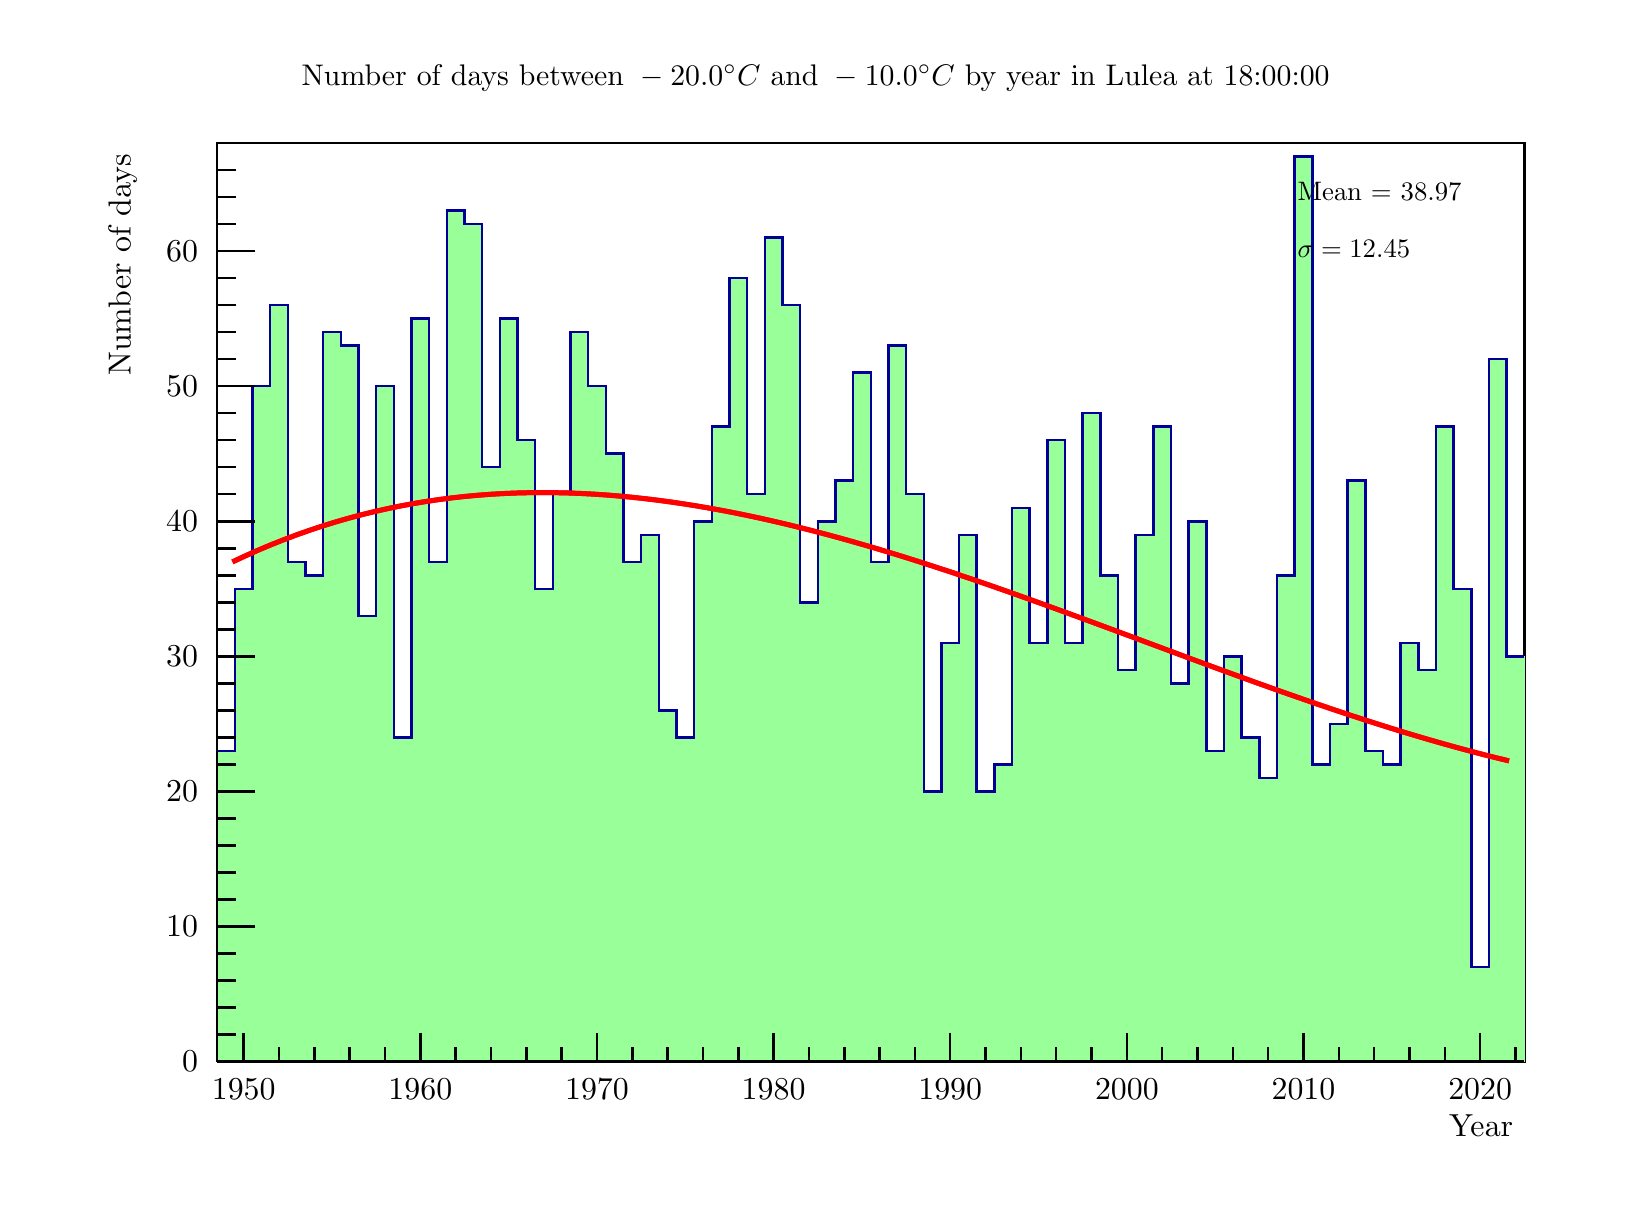
\begin{tikzpicture}
\def\CheckTikzLibraryLoaded#1{ \ifcsname tikz@library@#1@loaded\endcsname \else \PackageWarning{tikz}{usetikzlibrary{#1} is missing in the preamble.} \fi }
\CheckTikzLibraryLoaded{patterns}
\CheckTikzLibraryLoaded{plotmarks}
\pgfdeclareplotmark{cross} {
\pgfpathmoveto{\pgfpoint{-0.3\pgfplotmarksize}{\pgfplotmarksize}}
\pgfpathlineto{\pgfpoint{+0.3\pgfplotmarksize}{\pgfplotmarksize}}
\pgfpathlineto{\pgfpoint{+0.3\pgfplotmarksize}{0.3\pgfplotmarksize}}
\pgfpathlineto{\pgfpoint{+1\pgfplotmarksize}{0.3\pgfplotmarksize}}
\pgfpathlineto{\pgfpoint{+1\pgfplotmarksize}{-0.3\pgfplotmarksize}}
\pgfpathlineto{\pgfpoint{+0.3\pgfplotmarksize}{-0.3\pgfplotmarksize}}
\pgfpathlineto{\pgfpoint{+0.3\pgfplotmarksize}{-1.\pgfplotmarksize}}
\pgfpathlineto{\pgfpoint{-0.3\pgfplotmarksize}{-1.\pgfplotmarksize}}
\pgfpathlineto{\pgfpoint{-0.3\pgfplotmarksize}{-0.3\pgfplotmarksize}}
\pgfpathlineto{\pgfpoint{-1.\pgfplotmarksize}{-0.3\pgfplotmarksize}}
\pgfpathlineto{\pgfpoint{-1.\pgfplotmarksize}{0.3\pgfplotmarksize}}
\pgfpathlineto{\pgfpoint{-0.3\pgfplotmarksize}{0.3\pgfplotmarksize}}
\pgfpathclose
\pgfusepathqstroke
}
\pgfdeclareplotmark{cross*} {
\pgfpathmoveto{\pgfpoint{-0.3\pgfplotmarksize}{\pgfplotmarksize}}
\pgfpathlineto{\pgfpoint{+0.3\pgfplotmarksize}{\pgfplotmarksize}}
\pgfpathlineto{\pgfpoint{+0.3\pgfplotmarksize}{0.3\pgfplotmarksize}}
\pgfpathlineto{\pgfpoint{+1\pgfplotmarksize}{0.3\pgfplotmarksize}}
\pgfpathlineto{\pgfpoint{+1\pgfplotmarksize}{-0.3\pgfplotmarksize}}
\pgfpathlineto{\pgfpoint{+0.3\pgfplotmarksize}{-0.3\pgfplotmarksize}}
\pgfpathlineto{\pgfpoint{+0.3\pgfplotmarksize}{-1.\pgfplotmarksize}}
\pgfpathlineto{\pgfpoint{-0.3\pgfplotmarksize}{-1.\pgfplotmarksize}}
\pgfpathlineto{\pgfpoint{-0.3\pgfplotmarksize}{-0.3\pgfplotmarksize}}
\pgfpathlineto{\pgfpoint{-1.\pgfplotmarksize}{-0.3\pgfplotmarksize}}
\pgfpathlineto{\pgfpoint{-1.\pgfplotmarksize}{0.3\pgfplotmarksize}}
\pgfpathlineto{\pgfpoint{-0.3\pgfplotmarksize}{0.3\pgfplotmarksize}}
\pgfpathclose
\pgfusepathqfillstroke
}
\pgfdeclareplotmark{newstar} {
\pgfpathmoveto{\pgfqpoint{0pt}{\pgfplotmarksize}}
\pgfpathlineto{\pgfqpointpolar{44}{0.5\pgfplotmarksize}}
\pgfpathlineto{\pgfqpointpolar{18}{\pgfplotmarksize}}
\pgfpathlineto{\pgfqpointpolar{-20}{0.5\pgfplotmarksize}}
\pgfpathlineto{\pgfqpointpolar{-54}{\pgfplotmarksize}}
\pgfpathlineto{\pgfqpointpolar{-90}{0.5\pgfplotmarksize}}
\pgfpathlineto{\pgfqpointpolar{234}{\pgfplotmarksize}}
\pgfpathlineto{\pgfqpointpolar{198}{0.5\pgfplotmarksize}}
\pgfpathlineto{\pgfqpointpolar{162}{\pgfplotmarksize}}
\pgfpathlineto{\pgfqpointpolar{134}{0.5\pgfplotmarksize}}
\pgfpathclose
\pgfusepathqstroke
}
\pgfdeclareplotmark{newstar*} {
\pgfpathmoveto{\pgfqpoint{0pt}{\pgfplotmarksize}}
\pgfpathlineto{\pgfqpointpolar{44}{0.5\pgfplotmarksize}}
\pgfpathlineto{\pgfqpointpolar{18}{\pgfplotmarksize}}
\pgfpathlineto{\pgfqpointpolar{-20}{0.5\pgfplotmarksize}}
\pgfpathlineto{\pgfqpointpolar{-54}{\pgfplotmarksize}}
\pgfpathlineto{\pgfqpointpolar{-90}{0.5\pgfplotmarksize}}
\pgfpathlineto{\pgfqpointpolar{234}{\pgfplotmarksize}}
\pgfpathlineto{\pgfqpointpolar{198}{0.5\pgfplotmarksize}}
\pgfpathlineto{\pgfqpointpolar{162}{\pgfplotmarksize}}
\pgfpathlineto{\pgfqpointpolar{134}{0.5\pgfplotmarksize}}
\pgfpathclose
\pgfusepathqfillstroke
}
\definecolor{c}{rgb}{1,1,1};
\draw [color=c, fill=c] (0,0) rectangle (20,14.5819);
\draw [color=c, fill=c] (2.4,1.45819) rectangle (19,13.1237);
\definecolor{c}{rgb}{0,0,0};
\draw [c,line width=0.9] (2.4,1.45819) -- (2.4,13.1237) -- (19,13.1237) -- (19,1.45819) -- (2.4,1.45819);
\definecolor{c}{rgb}{1,1,1};
\draw [color=c, fill=c] (2.4,1.45819) rectangle (19,13.1237);
\definecolor{c}{rgb}{0,0,0};
\draw [c,line width=0.9] (2.4,1.45819) -- (2.4,13.1237) -- (19,13.1237) -- (19,1.45819) -- (2.4,1.45819);
\definecolor{c}{rgb}{0.6,1,0.6};
\draw [c, fill=c] (2.4,1.45819) -- (2.4,5.4039) -- (2.62432,5.4039) -- (2.62432,7.46252) -- (2.84865,7.46252) -- (2.84865,10.0358) -- (3.07297,10.0358) -- (3.07297,11.0651) -- (3.2973,11.0651) -- (3.2973,7.80563) -- (3.52162,7.80563) --
 (3.52162,7.63407) -- (3.74595,7.63407) -- (3.74595,10.722) -- (3.97027,10.722) -- (3.97027,10.5505) -- (4.19459,10.5505) -- (4.19459,7.11942) -- (4.41892,7.11942) -- (4.41892,10.0358) -- (4.64324,10.0358) -- (4.64324,5.57545) -- (4.86757,5.57545) --
 (4.86757,10.8936) -- (5.09189,10.8936) -- (5.09189,7.80563) -- (5.31622,7.80563) -- (5.31622,12.266) -- (5.54054,12.266) -- (5.54054,12.0944) -- (5.76486,12.0944) -- (5.76486,9.00649) -- (5.98919,9.00649) -- (5.98919,10.8936) -- (6.21351,10.8936) --
 (6.21351,9.3496) -- (6.43784,9.3496) -- (6.43784,7.46252) -- (6.66216,7.46252) -- (6.66216,8.66339) -- (6.88649,8.66339) -- (6.88649,10.722) -- (7.11081,10.722) -- (7.11081,10.0358) -- (7.33513,10.0358) -- (7.33513,9.17804) -- (7.55946,9.17804) --
 (7.55946,7.80563) -- (7.78378,7.80563) -- (7.78378,8.14873) -- (8.00811,8.14873) -- (8.00811,5.91855) -- (8.23243,5.91855) -- (8.23243,5.57545) -- (8.45676,5.57545) -- (8.45676,8.32028) -- (8.68108,8.32028) -- (8.68108,9.52115) -- (8.90541,9.52115)
 -- (8.90541,11.4082) -- (9.12973,11.4082) -- (9.12973,8.66339) -- (9.35405,8.66339) -- (9.35405,11.9229) -- (9.57838,11.9229) -- (9.57838,11.0651) -- (9.8027,11.0651) -- (9.8027,7.29097) -- (10.027,7.29097) -- (10.027,8.32028) -- (10.2514,8.32028)
 -- (10.2514,8.83494) -- (10.4757,8.83494) -- (10.4757,10.2074) -- (10.7,10.2074) -- (10.7,7.80563) -- (10.9243,7.80563) -- (10.9243,10.5505) -- (11.1486,10.5505) -- (11.1486,8.66339) -- (11.373,8.66339) -- (11.373,4.88924) -- (11.5973,4.88924) --
 (11.5973,6.77631) -- (11.8216,6.77631) -- (11.8216,8.14873) -- (12.0459,8.14873) -- (12.0459,4.88924) -- (12.2703,4.88924) -- (12.2703,5.23234) -- (12.4946,5.23234) -- (12.4946,8.49184) -- (12.7189,8.49184) -- (12.7189,6.77631) -- (12.9432,6.77631)
 -- (12.9432,9.3496) -- (13.1676,9.3496) -- (13.1676,6.77631) -- (13.3919,6.77631) -- (13.3919,9.6927) -- (13.6162,9.6927) -- (13.6162,7.63407) -- (13.8405,7.63407) -- (13.8405,6.43321) -- (14.0649,6.43321) -- (14.0649,8.14873) -- (14.2892,8.14873)
 -- (14.2892,9.52115) -- (14.5135,9.52115) -- (14.5135,6.26166) -- (14.7378,6.26166) -- (14.7378,8.32028) -- (14.9622,8.32028) -- (14.9622,5.4039) -- (15.1865,5.4039) -- (15.1865,6.60476) -- (15.4108,6.60476) -- (15.4108,5.57545) -- (15.6351,5.57545)
 -- (15.6351,5.06079) -- (15.8595,5.06079) -- (15.8595,7.63407) -- (16.0838,7.63407) -- (16.0838,12.9522) -- (16.3081,12.9522) -- (16.3081,5.23234) -- (16.5324,5.23234) -- (16.5324,5.747) -- (16.7568,5.747) -- (16.7568,8.83494) -- (16.9811,8.83494)
 -- (16.9811,5.4039) -- (17.2054,5.4039) -- (17.2054,5.23234) -- (17.4297,5.23234) -- (17.4297,6.77631) -- (17.6541,6.77631) -- (17.6541,6.43321) -- (17.8784,6.43321) -- (17.8784,9.52115) -- (18.1027,9.52115) -- (18.1027,7.46252) -- (18.327,7.46252)
 -- (18.327,2.65906) -- (18.5514,2.65906) -- (18.5514,10.3789) -- (18.7757,10.3789) -- (18.7757,6.60476) -- (19,6.60476) -- (19,1.45819);
\definecolor{c}{rgb}{0,0,0.6};
\draw [c,line width=0.9] (2.4,5.4039) -- (2.62432,5.4039) -- (2.62432,7.46252) -- (2.84865,7.46252) -- (2.84865,10.0358) -- (3.07297,10.0358) -- (3.07297,11.0651) -- (3.2973,11.0651) -- (3.2973,7.80563) -- (3.52162,7.80563) -- (3.52162,7.63407) --
 (3.74595,7.63407) -- (3.74595,10.722) -- (3.97027,10.722) -- (3.97027,10.5505) -- (4.19459,10.5505) -- (4.19459,7.11942) -- (4.41892,7.11942) -- (4.41892,10.0358) -- (4.64324,10.0358) -- (4.64324,5.57545) -- (4.86757,5.57545) -- (4.86757,10.8936) --
 (5.09189,10.8936) -- (5.09189,7.80563) -- (5.31622,7.80563) -- (5.31622,12.266) -- (5.54054,12.266) -- (5.54054,12.0944) -- (5.76486,12.0944) -- (5.76486,9.00649) -- (5.98919,9.00649) -- (5.98919,10.8936) -- (6.21351,10.8936) -- (6.21351,9.3496) --
 (6.43784,9.3496) -- (6.43784,7.46252) -- (6.66216,7.46252) -- (6.66216,8.66339) -- (6.88649,8.66339) -- (6.88649,10.722) -- (7.11081,10.722) -- (7.11081,10.0358) -- (7.33513,10.0358) -- (7.33513,9.17804) -- (7.55946,9.17804) -- (7.55946,7.80563) --
 (7.78378,7.80563) -- (7.78378,8.14873) -- (8.00811,8.14873) -- (8.00811,5.91855) -- (8.23243,5.91855) -- (8.23243,5.57545) -- (8.45676,5.57545) -- (8.45676,8.32028) -- (8.68108,8.32028) -- (8.68108,9.52115) -- (8.90541,9.52115) -- (8.90541,11.4082)
 -- (9.12973,11.4082) -- (9.12973,8.66339) -- (9.35405,8.66339) -- (9.35405,11.9229) -- (9.57838,11.9229) -- (9.57838,11.0651) -- (9.8027,11.0651) -- (9.8027,7.29097) -- (10.027,7.29097) -- (10.027,8.32028) -- (10.2514,8.32028) -- (10.2514,8.83494)
 -- (10.4757,8.83494) -- (10.4757,10.2074) -- (10.7,10.2074) -- (10.7,7.80563) -- (10.9243,7.80563) -- (10.9243,10.5505) -- (11.1486,10.5505) -- (11.1486,8.66339) -- (11.373,8.66339) -- (11.373,4.88924) -- (11.5973,4.88924) -- (11.5973,6.77631) --
 (11.8216,6.77631) -- (11.8216,8.14873) -- (12.0459,8.14873) -- (12.0459,4.88924) -- (12.2703,4.88924) -- (12.2703,5.23234) -- (12.4946,5.23234) -- (12.4946,8.49184) -- (12.7189,8.49184) -- (12.7189,6.77631) -- (12.9432,6.77631) -- (12.9432,9.3496)
 -- (13.1676,9.3496) -- (13.1676,6.77631) -- (13.3919,6.77631) -- (13.3919,9.6927) -- (13.6162,9.6927) -- (13.6162,7.63407) -- (13.8405,7.63407) -- (13.8405,6.43321) -- (14.0649,6.43321) -- (14.0649,8.14873) -- (14.2892,8.14873) -- (14.2892,9.52115)
 -- (14.5135,9.52115) -- (14.5135,6.26166) -- (14.7378,6.26166) -- (14.7378,8.32028) -- (14.9622,8.32028) -- (14.9622,5.4039) -- (15.1865,5.4039) -- (15.1865,6.60476) -- (15.4108,6.60476) -- (15.4108,5.57545) -- (15.6351,5.57545) -- (15.6351,5.06079)
 -- (15.8595,5.06079) -- (15.8595,7.63407) -- (16.0838,7.63407) -- (16.0838,12.9522) -- (16.3081,12.9522) -- (16.3081,5.23234) -- (16.5324,5.23234) -- (16.5324,5.747) -- (16.7568,5.747) -- (16.7568,8.83494) -- (16.9811,8.83494) -- (16.9811,5.4039) --
 (17.2054,5.4039) -- (17.2054,5.23234) -- (17.4297,5.23234) -- (17.4297,6.77631) -- (17.6541,6.77631) -- (17.6541,6.43321) -- (17.8784,6.43321) -- (17.8784,9.52115) -- (18.1027,9.52115) -- (18.1027,7.46252) -- (18.327,7.46252) -- (18.327,2.65906) --
 (18.5514,2.65906) -- (18.5514,10.3789) -- (18.7757,10.3789) -- (18.7757,6.60476) -- (19,6.60476);
\definecolor{c}{rgb}{1,0,0};
\draw [c,line width=1.8] (2.59404,7.80429) -- (2.7578,7.88089) -- (2.92155,7.95361) -- (3.08531,8.0225) -- (3.24907,8.08763) -- (3.41282,8.14905) -- (3.57658,8.20681) -- (3.74034,8.26097) -- (3.90409,8.31159) -- (4.06785,8.35871) -- (4.23161,8.4024)
 -- (4.39536,8.44272) -- (4.55912,8.4797) -- (4.72288,8.51343) -- (4.88664,8.54393) -- (5.05039,8.57129) -- (5.21415,8.59554) -- (5.37791,8.61674) -- (5.54166,8.63496) -- (5.70542,8.65024) -- (5.86918,8.66264) -- (6.03293,8.67221) --
 (6.19669,8.67902) -- (6.36045,8.68312) -- (6.5242,8.68455) -- (6.68796,8.68339) -- (6.85172,8.67968) -- (7.01547,8.67348) -- (7.17923,8.66484) -- (7.34299,8.65382) -- (7.50674,8.64048) -- (7.6705,8.62487) -- (7.83426,8.60704) -- (7.99801,8.58706) --
 (8.16177,8.56497) -- (8.32553,8.54084) -- (8.48928,8.51471) -- (8.65304,8.48665) -- (8.8168,8.45671) -- (8.98055,8.42494) -- (9.14431,8.39141) -- (9.30807,8.35616) -- (9.47182,8.31925) -- (9.63558,8.28073) -- (9.79934,8.24067) -- (9.96309,8.19912)
 -- (10.1269,8.15613) -- (10.2906,8.11175) -- (10.4544,8.06606) -- (10.6181,8.01909);
\draw [c,line width=1.8] (10.6181,8.01909) -- (10.7819,7.97091) -- (10.9456,7.92156) -- (11.1094,7.87112) -- (11.2731,7.81962) -- (11.4369,7.76713) -- (11.6007,7.71371) -- (11.7644,7.6594) -- (11.9282,7.60427) -- (12.0919,7.54836) --
 (12.2557,7.49174) -- (12.4194,7.43446) -- (12.5832,7.37657) -- (12.747,7.31814) -- (12.9107,7.25921) -- (13.0745,7.19984) -- (13.2382,7.14009) -- (13.402,7.08002) -- (13.5657,7.01967) -- (13.7295,6.9591) -- (13.8933,6.89838) -- (14.057,6.83755) --
 (14.2208,6.77667) -- (14.3845,6.71579) -- (14.5483,6.65498) -- (14.712,6.59428) -- (14.8758,6.53375) -- (15.0396,6.47346) -- (15.2033,6.41344) -- (15.3671,6.35377) -- (15.5308,6.29448) -- (15.6946,6.23565) -- (15.8583,6.17732) -- (16.0221,6.11956)
 -- (16.1859,6.0624) -- (16.3496,6.00593) -- (16.5134,5.95017) -- (16.6771,5.8952) -- (16.8409,5.84107) -- (17.0046,5.78783) -- (17.1684,5.73554) -- (17.3321,5.68425) -- (17.4959,5.63403) -- (17.6597,5.58492) -- (17.8234,5.53698) -- (17.9872,5.49026)
 -- (18.1509,5.44483) -- (18.3147,5.40074) -- (18.4784,5.35803) -- (18.6422,5.31678);
\draw [c,line width=1.8] (18.6422,5.31678) -- (18.806,5.27703);
\definecolor{c}{rgb}{0,0,0};
\draw [c,line width=0.9] (2.4,1.45819) -- (19,1.45819);
\draw [c,line width=0.9] (2.73649,1.82128) -- (2.73649,1.45819);
\draw [c,line width=0.9] (3.18514,1.63974) -- (3.18514,1.45819);
\draw [c,line width=0.9] (3.63378,1.63974) -- (3.63378,1.45819);
\draw [c,line width=0.9] (4.08243,1.63974) -- (4.08243,1.45819);
\draw [c,line width=0.9] (4.53108,1.63974) -- (4.53108,1.45819);
\draw [c,line width=0.9] (4.97973,1.82128) -- (4.97973,1.45819);
\draw [c,line width=0.9] (5.42838,1.63974) -- (5.42838,1.45819);
\draw [c,line width=0.9] (5.87703,1.63974) -- (5.87703,1.45819);
\draw [c,line width=0.9] (6.32568,1.63974) -- (6.32568,1.45819);
\draw [c,line width=0.9] (6.77432,1.63974) -- (6.77432,1.45819);
\draw [c,line width=0.9] (7.22297,1.82128) -- (7.22297,1.45819);
\draw [c,line width=0.9] (7.67162,1.63974) -- (7.67162,1.45819);
\draw [c,line width=0.9] (8.12027,1.63974) -- (8.12027,1.45819);
\draw [c,line width=0.9] (8.56892,1.63974) -- (8.56892,1.45819);
\draw [c,line width=0.9] (9.01757,1.63974) -- (9.01757,1.45819);
\draw [c,line width=0.9] (9.46622,1.82128) -- (9.46622,1.45819);
\draw [c,line width=0.9] (9.91486,1.63974) -- (9.91486,1.45819);
\draw [c,line width=0.9] (10.3635,1.63974) -- (10.3635,1.45819);
\draw [c,line width=0.9] (10.8122,1.63974) -- (10.8122,1.45819);
\draw [c,line width=0.9] (11.2608,1.63974) -- (11.2608,1.45819);
\draw [c,line width=0.9] (11.7095,1.82128) -- (11.7095,1.45819);
\draw [c,line width=0.9] (12.1581,1.63974) -- (12.1581,1.45819);
\draw [c,line width=0.9] (12.6068,1.63974) -- (12.6068,1.45819);
\draw [c,line width=0.9] (13.0554,1.63974) -- (13.0554,1.45819);
\draw [c,line width=0.9] (13.5041,1.63974) -- (13.5041,1.45819);
\draw [c,line width=0.9] (13.9527,1.82128) -- (13.9527,1.45819);
\draw [c,line width=0.9] (14.4014,1.63974) -- (14.4014,1.45819);
\draw [c,line width=0.9] (14.85,1.63974) -- (14.85,1.45819);
\draw [c,line width=0.9] (15.2986,1.63974) -- (15.2986,1.45819);
\draw [c,line width=0.9] (15.7473,1.63974) -- (15.7473,1.45819);
\draw [c,line width=0.9] (16.1959,1.82128) -- (16.1959,1.45819);
\draw [c,line width=0.9] (16.6446,1.63974) -- (16.6446,1.45819);
\draw [c,line width=0.9] (17.0932,1.63974) -- (17.0932,1.45819);
\draw [c,line width=0.9] (17.5419,1.63974) -- (17.5419,1.45819);
\draw [c,line width=0.9] (17.9905,1.63974) -- (17.9905,1.45819);
\draw [c,line width=0.9] (18.4392,1.82128) -- (18.4392,1.45819);
\draw [c,line width=0.9] (2.73649,1.82128) -- (2.73649,1.45819);
\draw [c,line width=0.9] (18.4392,1.82128) -- (18.4392,1.45819);
\draw [c,line width=0.9] (18.8878,1.63974) -- (18.8878,1.45819);
\draw [anchor=base] (2.73649,0.97699) node[scale=1.15134, color=c, rotate=0]{1950};
\draw [anchor=base] (4.97973,0.97699) node[scale=1.15134, color=c, rotate=0]{1960};
\draw [anchor=base] (7.22297,0.97699) node[scale=1.15134, color=c, rotate=0]{1970};
\draw [anchor=base] (9.46622,0.97699) node[scale=1.15134, color=c, rotate=0]{1980};
\draw [anchor=base] (11.7095,0.97699) node[scale=1.15134, color=c, rotate=0]{1990};
\draw [anchor=base] (13.9527,0.97699) node[scale=1.15134, color=c, rotate=0]{2000};
\draw [anchor=base] (16.1959,0.97699) node[scale=1.15134, color=c, rotate=0]{2010};
\draw [anchor=base] (18.4392,0.97699) node[scale=1.15134, color=c, rotate=0]{2020};
\draw [anchor= east] (19,0.641605) node[scale=1.15134, color=c, rotate=0]{Year};
\draw [c,line width=0.9] (2.4,1.45819) -- (2.4,13.1237);
\draw [c,line width=0.9] (2.88,1.45819) -- (2.4,1.45819);
\draw [c,line width=0.9] (2.64,1.8013) -- (2.4,1.8013);
\draw [c,line width=0.9] (2.64,2.1444) -- (2.4,2.1444);
\draw [c,line width=0.9] (2.64,2.48751) -- (2.4,2.48751);
\draw [c,line width=0.9] (2.64,2.83061) -- (2.4,2.83061);
\draw [c,line width=0.9] (2.88,3.17372) -- (2.4,3.17372);
\draw [c,line width=0.9] (2.64,3.51682) -- (2.4,3.51682);
\draw [c,line width=0.9] (2.64,3.85993) -- (2.4,3.85993);
\draw [c,line width=0.9] (2.64,4.20303) -- (2.4,4.20303);
\draw [c,line width=0.9] (2.64,4.54613) -- (2.4,4.54613);
\draw [c,line width=0.9] (2.88,4.88924) -- (2.4,4.88924);
\draw [c,line width=0.9] (2.64,5.23234) -- (2.4,5.23234);
\draw [c,line width=0.9] (2.64,5.57545) -- (2.4,5.57545);
\draw [c,line width=0.9] (2.64,5.91855) -- (2.4,5.91855);
\draw [c,line width=0.9] (2.64,6.26166) -- (2.4,6.26166);
\draw [c,line width=0.9] (2.88,6.60476) -- (2.4,6.60476);
\draw [c,line width=0.9] (2.64,6.94787) -- (2.4,6.94787);
\draw [c,line width=0.9] (2.64,7.29097) -- (2.4,7.29097);
\draw [c,line width=0.9] (2.64,7.63407) -- (2.4,7.63407);
\draw [c,line width=0.9] (2.64,7.97718) -- (2.4,7.97718);
\draw [c,line width=0.9] (2.88,8.32028) -- (2.4,8.32028);
\draw [c,line width=0.9] (2.64,8.66339) -- (2.4,8.66339);
\draw [c,line width=0.9] (2.64,9.00649) -- (2.4,9.00649);
\draw [c,line width=0.9] (2.64,9.3496) -- (2.4,9.3496);
\draw [c,line width=0.9] (2.64,9.6927) -- (2.4,9.6927);
\draw [c,line width=0.9] (2.88,10.0358) -- (2.4,10.0358);
\draw [c,line width=0.9] (2.64,10.3789) -- (2.4,10.3789);
\draw [c,line width=0.9] (2.64,10.722) -- (2.4,10.722);
\draw [c,line width=0.9] (2.64,11.0651) -- (2.4,11.0651);
\draw [c,line width=0.9] (2.64,11.4082) -- (2.4,11.4082);
\draw [c,line width=0.9] (2.88,11.7513) -- (2.4,11.7513);
\draw [c,line width=0.9] (2.88,11.7513) -- (2.4,11.7513);
\draw [c,line width=0.9] (2.64,12.0944) -- (2.4,12.0944);
\draw [c,line width=0.9] (2.64,12.4375) -- (2.4,12.4375);
\draw [c,line width=0.9] (2.64,12.7806) -- (2.4,12.7806);
\draw [c,line width=0.9] (2.64,13.1237) -- (2.4,13.1237);
\draw [anchor= east] (2.3,1.45819) node[scale=1.15134, color=c, rotate=0]{0};
\draw [anchor= east] (2.3,3.17372) node[scale=1.15134, color=c, rotate=0]{10};
\draw [anchor= east] (2.3,4.88924) node[scale=1.15134, color=c, rotate=0]{20};
\draw [anchor= east] (2.3,6.60476) node[scale=1.15134, color=c, rotate=0]{30};
\draw [anchor= east] (2.3,8.32028) node[scale=1.15134, color=c, rotate=0]{40};
\draw [anchor= east] (2.3,10.0358) node[scale=1.15134, color=c, rotate=0]{50};
\draw [anchor= east] (2.3,11.7513) node[scale=1.15134, color=c, rotate=0]{60};
\draw [anchor= east] (1.19833,13.1237) node[scale=1.15134, color=c, rotate=90]{Number of days};
\definecolor{c}{rgb}{1,0,0};
\draw [c,line width=1.8] (2.59404,7.80429) -- (2.7578,7.88089) -- (2.92155,7.95361) -- (3.08531,8.0225) -- (3.24907,8.08763) -- (3.41282,8.14905) -- (3.57658,8.20681) -- (3.74034,8.26097) -- (3.90409,8.31159) -- (4.06785,8.35871) -- (4.23161,8.4024)
 -- (4.39536,8.44272) -- (4.55912,8.4797) -- (4.72288,8.51343) -- (4.88664,8.54393) -- (5.05039,8.57129) -- (5.21415,8.59554) -- (5.37791,8.61674) -- (5.54166,8.63496) -- (5.70542,8.65024) -- (5.86918,8.66264) -- (6.03293,8.67221) --
 (6.19669,8.67902) -- (6.36045,8.68312) -- (6.5242,8.68455) -- (6.68796,8.68339) -- (6.85172,8.67968) -- (7.01547,8.67348) -- (7.17923,8.66484) -- (7.34299,8.65382) -- (7.50674,8.64048) -- (7.6705,8.62487) -- (7.83426,8.60704) -- (7.99801,8.58706) --
 (8.16177,8.56497) -- (8.32553,8.54084) -- (8.48928,8.51471) -- (8.65304,8.48665) -- (8.8168,8.45671) -- (8.98055,8.42494) -- (9.14431,8.39141) -- (9.30807,8.35616) -- (9.47182,8.31925) -- (9.63558,8.28073) -- (9.79934,8.24067) -- (9.96309,8.19912)
 -- (10.1269,8.15613) -- (10.2906,8.11175) -- (10.4544,8.06606) -- (10.6181,8.01909);
\draw [c,line width=1.8] (10.6181,8.01909) -- (10.7819,7.97091) -- (10.9456,7.92156) -- (11.1094,7.87112) -- (11.2731,7.81962) -- (11.4369,7.76713) -- (11.6007,7.71371) -- (11.7644,7.6594) -- (11.9282,7.60427) -- (12.0919,7.54836) --
 (12.2557,7.49174) -- (12.4194,7.43446) -- (12.5832,7.37657) -- (12.747,7.31814) -- (12.9107,7.25921) -- (13.0745,7.19984) -- (13.2382,7.14009) -- (13.402,7.08002) -- (13.5657,7.01967) -- (13.7295,6.9591) -- (13.8933,6.89838) -- (14.057,6.83755) --
 (14.2208,6.77667) -- (14.3845,6.71579) -- (14.5483,6.65498) -- (14.712,6.59428) -- (14.8758,6.53375) -- (15.0396,6.47346) -- (15.2033,6.41344) -- (15.3671,6.35377) -- (15.5308,6.29448) -- (15.6946,6.23565) -- (15.8583,6.17732) -- (16.0221,6.11956)
 -- (16.1859,6.0624) -- (16.3496,6.00593) -- (16.5134,5.95017) -- (16.6771,5.8952) -- (16.8409,5.84107) -- (17.0046,5.78783) -- (17.1684,5.73554) -- (17.3321,5.68425) -- (17.4959,5.63403) -- (17.6597,5.58492) -- (17.8234,5.53698) -- (17.9872,5.49026)
 -- (18.1509,5.44483) -- (18.3147,5.40074) -- (18.4784,5.35803) -- (18.6422,5.31678);
\draw [c,line width=1.8] (18.6422,5.31678) -- (18.806,5.27703);
\definecolor{c}{rgb}{0,0,0};
\draw [anchor=base west] (16,12.3946) node[scale=0.965639, color=c, rotate=0]{Mean = 38.97};
\draw [anchor=base west] (16,11.6656) node[scale=0.965639, color=c, rotate=0]{$\sigma = 12.45$};
\draw (10,13.9476) node[scale=1.07706, color=c, rotate=0]{$\text{Number of days between }-20.0^{\circ}C\text{ and }-10.0^{\circ}C\text{ by year in }\text{Lulea at 18:00:00}$};
\end{tikzpicture}
%\end{document}
}
    \label{fig:enter-label}
\end{figure}

Also in Luleå, two consecutive years had a 7-day streak of temperatures within half-a-degree Celsius at midnight. No other years saw such a long streak of similar temperatures.

\begin{figure}[H]
    \centering
    \scalebox{.5}{%\documentclass{standalone}
%\usepackage{tikz}
%\usetikzlibrary{patterns,plotmarks}
%\begin{document}
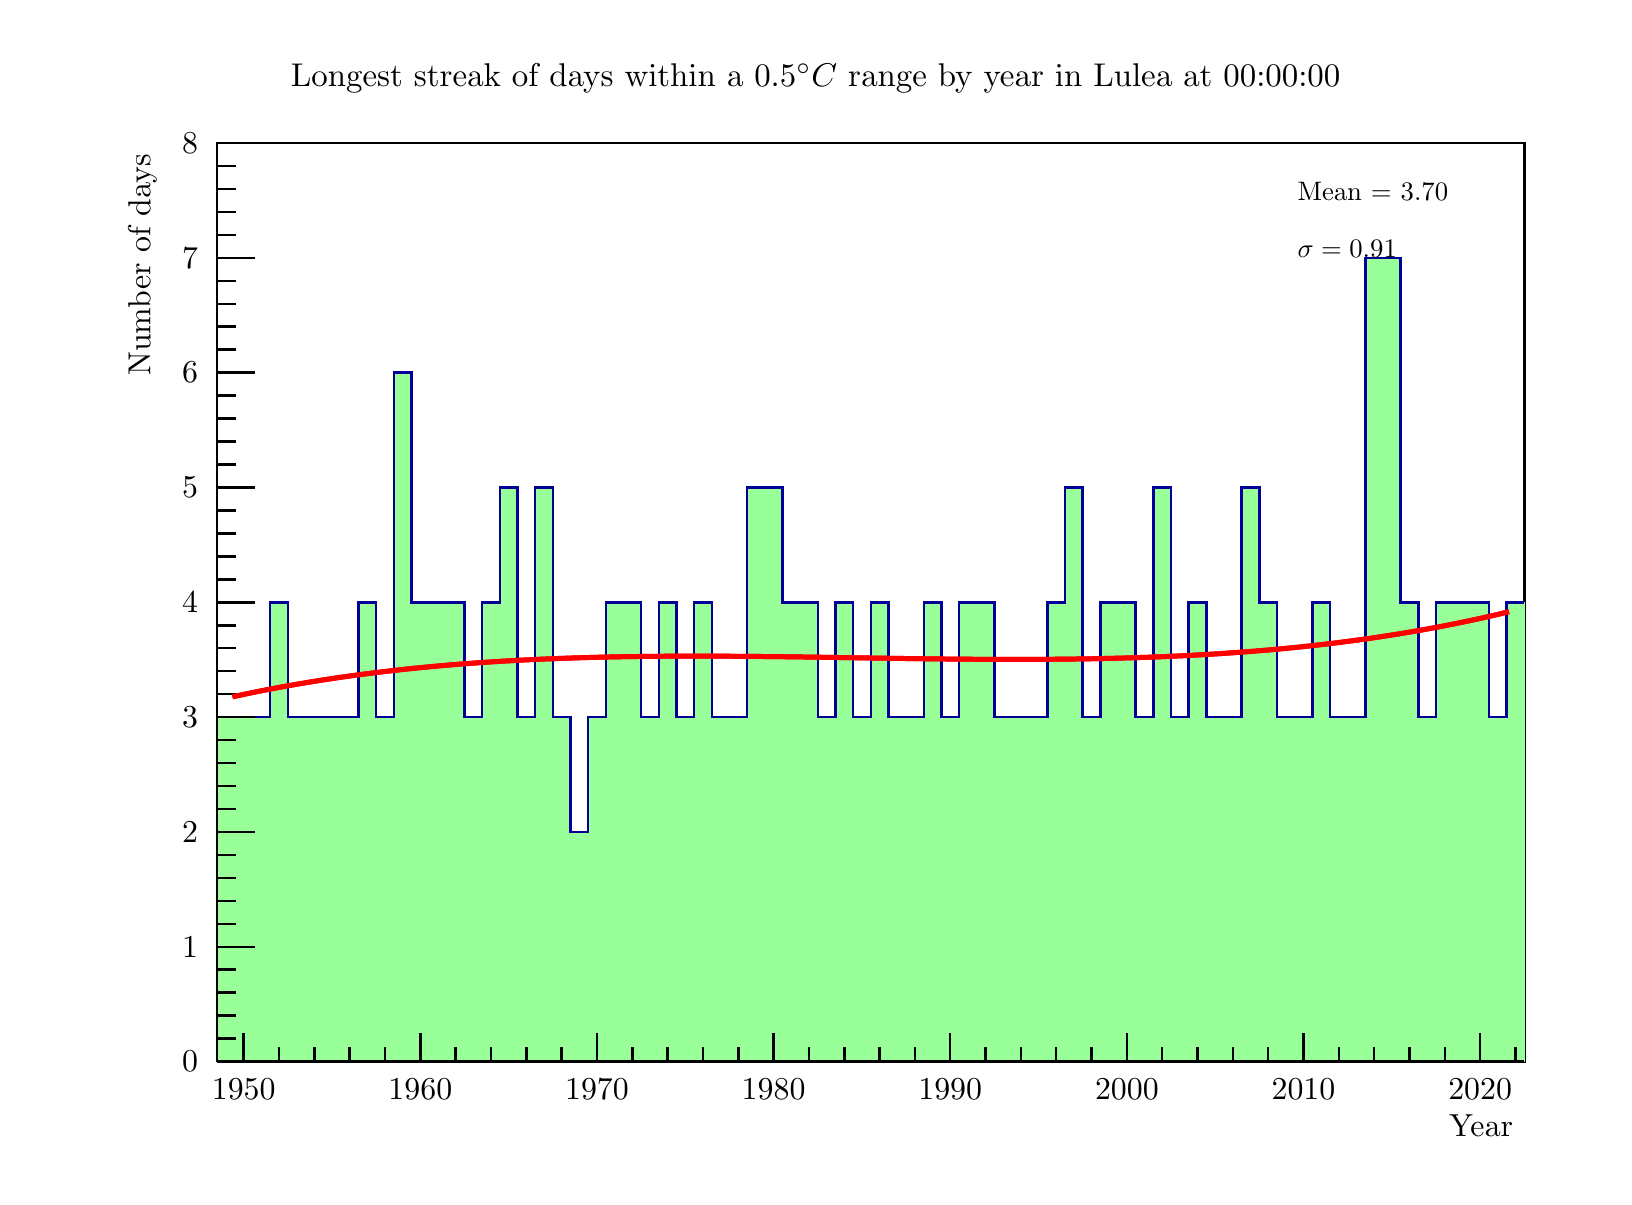
\begin{tikzpicture}
\def\CheckTikzLibraryLoaded#1{ \ifcsname tikz@library@#1@loaded\endcsname \else \PackageWarning{tikz}{usetikzlibrary{#1} is missing in the preamble.} \fi }
\CheckTikzLibraryLoaded{patterns}
\CheckTikzLibraryLoaded{plotmarks}
\pgfdeclareplotmark{cross} {
\pgfpathmoveto{\pgfpoint{-0.3\pgfplotmarksize}{\pgfplotmarksize}}
\pgfpathlineto{\pgfpoint{+0.3\pgfplotmarksize}{\pgfplotmarksize}}
\pgfpathlineto{\pgfpoint{+0.3\pgfplotmarksize}{0.3\pgfplotmarksize}}
\pgfpathlineto{\pgfpoint{+1\pgfplotmarksize}{0.3\pgfplotmarksize}}
\pgfpathlineto{\pgfpoint{+1\pgfplotmarksize}{-0.3\pgfplotmarksize}}
\pgfpathlineto{\pgfpoint{+0.3\pgfplotmarksize}{-0.3\pgfplotmarksize}}
\pgfpathlineto{\pgfpoint{+0.3\pgfplotmarksize}{-1.\pgfplotmarksize}}
\pgfpathlineto{\pgfpoint{-0.3\pgfplotmarksize}{-1.\pgfplotmarksize}}
\pgfpathlineto{\pgfpoint{-0.3\pgfplotmarksize}{-0.3\pgfplotmarksize}}
\pgfpathlineto{\pgfpoint{-1.\pgfplotmarksize}{-0.3\pgfplotmarksize}}
\pgfpathlineto{\pgfpoint{-1.\pgfplotmarksize}{0.3\pgfplotmarksize}}
\pgfpathlineto{\pgfpoint{-0.3\pgfplotmarksize}{0.3\pgfplotmarksize}}
\pgfpathclose
\pgfusepathqstroke
}
\pgfdeclareplotmark{cross*} {
\pgfpathmoveto{\pgfpoint{-0.3\pgfplotmarksize}{\pgfplotmarksize}}
\pgfpathlineto{\pgfpoint{+0.3\pgfplotmarksize}{\pgfplotmarksize}}
\pgfpathlineto{\pgfpoint{+0.3\pgfplotmarksize}{0.3\pgfplotmarksize}}
\pgfpathlineto{\pgfpoint{+1\pgfplotmarksize}{0.3\pgfplotmarksize}}
\pgfpathlineto{\pgfpoint{+1\pgfplotmarksize}{-0.3\pgfplotmarksize}}
\pgfpathlineto{\pgfpoint{+0.3\pgfplotmarksize}{-0.3\pgfplotmarksize}}
\pgfpathlineto{\pgfpoint{+0.3\pgfplotmarksize}{-1.\pgfplotmarksize}}
\pgfpathlineto{\pgfpoint{-0.3\pgfplotmarksize}{-1.\pgfplotmarksize}}
\pgfpathlineto{\pgfpoint{-0.3\pgfplotmarksize}{-0.3\pgfplotmarksize}}
\pgfpathlineto{\pgfpoint{-1.\pgfplotmarksize}{-0.3\pgfplotmarksize}}
\pgfpathlineto{\pgfpoint{-1.\pgfplotmarksize}{0.3\pgfplotmarksize}}
\pgfpathlineto{\pgfpoint{-0.3\pgfplotmarksize}{0.3\pgfplotmarksize}}
\pgfpathclose
\pgfusepathqfillstroke
}
\pgfdeclareplotmark{newstar} {
\pgfpathmoveto{\pgfqpoint{0pt}{\pgfplotmarksize}}
\pgfpathlineto{\pgfqpointpolar{44}{0.5\pgfplotmarksize}}
\pgfpathlineto{\pgfqpointpolar{18}{\pgfplotmarksize}}
\pgfpathlineto{\pgfqpointpolar{-20}{0.5\pgfplotmarksize}}
\pgfpathlineto{\pgfqpointpolar{-54}{\pgfplotmarksize}}
\pgfpathlineto{\pgfqpointpolar{-90}{0.5\pgfplotmarksize}}
\pgfpathlineto{\pgfqpointpolar{234}{\pgfplotmarksize}}
\pgfpathlineto{\pgfqpointpolar{198}{0.5\pgfplotmarksize}}
\pgfpathlineto{\pgfqpointpolar{162}{\pgfplotmarksize}}
\pgfpathlineto{\pgfqpointpolar{134}{0.5\pgfplotmarksize}}
\pgfpathclose
\pgfusepathqstroke
}
\pgfdeclareplotmark{newstar*} {
\pgfpathmoveto{\pgfqpoint{0pt}{\pgfplotmarksize}}
\pgfpathlineto{\pgfqpointpolar{44}{0.5\pgfplotmarksize}}
\pgfpathlineto{\pgfqpointpolar{18}{\pgfplotmarksize}}
\pgfpathlineto{\pgfqpointpolar{-20}{0.5\pgfplotmarksize}}
\pgfpathlineto{\pgfqpointpolar{-54}{\pgfplotmarksize}}
\pgfpathlineto{\pgfqpointpolar{-90}{0.5\pgfplotmarksize}}
\pgfpathlineto{\pgfqpointpolar{234}{\pgfplotmarksize}}
\pgfpathlineto{\pgfqpointpolar{198}{0.5\pgfplotmarksize}}
\pgfpathlineto{\pgfqpointpolar{162}{\pgfplotmarksize}}
\pgfpathlineto{\pgfqpointpolar{134}{0.5\pgfplotmarksize}}
\pgfpathclose
\pgfusepathqfillstroke
}
\definecolor{c}{rgb}{1,1,1};
\draw [color=c, fill=c] (0,0) rectangle (20,14.5819);
\draw [color=c, fill=c] (2.4,1.45819) rectangle (19,13.1237);
\definecolor{c}{rgb}{0,0,0};
\draw [c,line width=0.9] (2.4,1.45819) -- (2.4,13.1237) -- (19,13.1237) -- (19,1.45819) -- (2.4,1.45819);
\definecolor{c}{rgb}{1,1,1};
\draw [color=c, fill=c] (2.4,1.45819) rectangle (19,13.1237);
\definecolor{c}{rgb}{0,0,0};
\draw [c,line width=0.9] (2.4,1.45819) -- (2.4,13.1237) -- (19,13.1237) -- (19,1.45819) -- (2.4,1.45819);
\definecolor{c}{rgb}{0.6,1,0.6};
\draw [c, fill=c] (2.4,1.45819) -- (2.4,5.83278) -- (2.62432,5.83278) -- (2.62432,5.83278) -- (2.84865,5.83278) -- (2.84865,5.83278) -- (3.07297,5.83278) -- (3.07297,7.29097) -- (3.2973,7.29097) -- (3.2973,5.83278) -- (3.52162,5.83278) --
 (3.52162,5.83278) -- (3.74595,5.83278) -- (3.74595,5.83278) -- (3.97027,5.83278) -- (3.97027,5.83278) -- (4.19459,5.83278) -- (4.19459,7.29097) -- (4.41892,7.29097) -- (4.41892,5.83278) -- (4.64324,5.83278) -- (4.64324,10.2074) -- (4.86757,10.2074)
 -- (4.86757,7.29097) -- (5.09189,7.29097) -- (5.09189,7.29097) -- (5.31622,7.29097) -- (5.31622,7.29097) -- (5.54054,7.29097) -- (5.54054,5.83278) -- (5.76486,5.83278) -- (5.76486,7.29097) -- (5.98919,7.29097) -- (5.98919,8.74916) --
 (6.21351,8.74916) -- (6.21351,5.83278) -- (6.43784,5.83278) -- (6.43784,8.74916) -- (6.66216,8.74916) -- (6.66216,5.83278) -- (6.88649,5.83278) -- (6.88649,4.37458) -- (7.11081,4.37458) -- (7.11081,5.83278) -- (7.33513,5.83278) -- (7.33513,7.29097)
 -- (7.55946,7.29097) -- (7.55946,7.29097) -- (7.78378,7.29097) -- (7.78378,5.83278) -- (8.00811,5.83278) -- (8.00811,7.29097) -- (8.23243,7.29097) -- (8.23243,5.83278) -- (8.45676,5.83278) -- (8.45676,7.29097) -- (8.68108,7.29097) --
 (8.68108,5.83278) -- (8.90541,5.83278) -- (8.90541,5.83278) -- (9.12973,5.83278) -- (9.12973,8.74916) -- (9.35405,8.74916) -- (9.35405,8.74916) -- (9.57838,8.74916) -- (9.57838,7.29097) -- (9.8027,7.29097) -- (9.8027,7.29097) -- (10.027,7.29097) --
 (10.027,5.83278) -- (10.2514,5.83278) -- (10.2514,7.29097) -- (10.4757,7.29097) -- (10.4757,5.83278) -- (10.7,5.83278) -- (10.7,7.29097) -- (10.9243,7.29097) -- (10.9243,5.83278) -- (11.1486,5.83278) -- (11.1486,5.83278) -- (11.373,5.83278) --
 (11.373,7.29097) -- (11.5973,7.29097) -- (11.5973,5.83278) -- (11.8216,5.83278) -- (11.8216,7.29097) -- (12.0459,7.29097) -- (12.0459,7.29097) -- (12.2703,7.29097) -- (12.2703,5.83278) -- (12.4946,5.83278) -- (12.4946,5.83278) -- (12.7189,5.83278)
 -- (12.7189,5.83278) -- (12.9432,5.83278) -- (12.9432,7.29097) -- (13.1676,7.29097) -- (13.1676,8.74916) -- (13.3919,8.74916) -- (13.3919,5.83278) -- (13.6162,5.83278) -- (13.6162,7.29097) -- (13.8405,7.29097) -- (13.8405,7.29097) --
 (14.0649,7.29097) -- (14.0649,5.83278) -- (14.2892,5.83278) -- (14.2892,8.74916) -- (14.5135,8.74916) -- (14.5135,5.83278) -- (14.7378,5.83278) -- (14.7378,7.29097) -- (14.9622,7.29097) -- (14.9622,5.83278) -- (15.1865,5.83278) -- (15.1865,5.83278)
 -- (15.4108,5.83278) -- (15.4108,8.74916) -- (15.6351,8.74916) -- (15.6351,7.29097) -- (15.8595,7.29097) -- (15.8595,5.83278) -- (16.0838,5.83278) -- (16.0838,5.83278) -- (16.3081,5.83278) -- (16.3081,7.29097) -- (16.5324,7.29097) --
 (16.5324,5.83278) -- (16.7568,5.83278) -- (16.7568,5.83278) -- (16.9811,5.83278) -- (16.9811,11.6656) -- (17.2054,11.6656) -- (17.2054,11.6656) -- (17.4297,11.6656) -- (17.4297,7.29097) -- (17.6541,7.29097) -- (17.6541,5.83278) -- (17.8784,5.83278)
 -- (17.8784,7.29097) -- (18.1027,7.29097) -- (18.1027,7.29097) -- (18.327,7.29097) -- (18.327,7.29097) -- (18.5514,7.29097) -- (18.5514,5.83278) -- (18.7757,5.83278) -- (18.7757,7.29097) -- (19,7.29097) -- (19,1.45819);
\definecolor{c}{rgb}{0,0,0.6};
\draw [c,line width=0.9] (2.4,5.83278) -- (2.62432,5.83278) -- (2.62432,5.83278) -- (2.84865,5.83278) -- (2.84865,5.83278) -- (3.07297,5.83278) -- (3.07297,7.29097) -- (3.2973,7.29097) -- (3.2973,5.83278) -- (3.52162,5.83278) -- (3.52162,5.83278) --
 (3.74595,5.83278) -- (3.74595,5.83278) -- (3.97027,5.83278) -- (3.97027,5.83278) -- (4.19459,5.83278) -- (4.19459,7.29097) -- (4.41892,7.29097) -- (4.41892,5.83278) -- (4.64324,5.83278) -- (4.64324,10.2074) -- (4.86757,10.2074) -- (4.86757,7.29097)
 -- (5.09189,7.29097) -- (5.09189,7.29097) -- (5.31622,7.29097) -- (5.31622,7.29097) -- (5.54054,7.29097) -- (5.54054,5.83278) -- (5.76486,5.83278) -- (5.76486,7.29097) -- (5.98919,7.29097) -- (5.98919,8.74916) -- (6.21351,8.74916) --
 (6.21351,5.83278) -- (6.43784,5.83278) -- (6.43784,8.74916) -- (6.66216,8.74916) -- (6.66216,5.83278) -- (6.88649,5.83278) -- (6.88649,4.37458) -- (7.11081,4.37458) -- (7.11081,5.83278) -- (7.33513,5.83278) -- (7.33513,7.29097) -- (7.55946,7.29097)
 -- (7.55946,7.29097) -- (7.78378,7.29097) -- (7.78378,5.83278) -- (8.00811,5.83278) -- (8.00811,7.29097) -- (8.23243,7.29097) -- (8.23243,5.83278) -- (8.45676,5.83278) -- (8.45676,7.29097) -- (8.68108,7.29097) -- (8.68108,5.83278) --
 (8.90541,5.83278) -- (8.90541,5.83278) -- (9.12973,5.83278) -- (9.12973,8.74916) -- (9.35405,8.74916) -- (9.35405,8.74916) -- (9.57838,8.74916) -- (9.57838,7.29097) -- (9.8027,7.29097) -- (9.8027,7.29097) -- (10.027,7.29097) -- (10.027,5.83278) --
 (10.2514,5.83278) -- (10.2514,7.29097) -- (10.4757,7.29097) -- (10.4757,5.83278) -- (10.7,5.83278) -- (10.7,7.29097) -- (10.9243,7.29097) -- (10.9243,5.83278) -- (11.1486,5.83278) -- (11.1486,5.83278) -- (11.373,5.83278) -- (11.373,7.29097) --
 (11.5973,7.29097) -- (11.5973,5.83278) -- (11.8216,5.83278) -- (11.8216,7.29097) -- (12.0459,7.29097) -- (12.0459,7.29097) -- (12.2703,7.29097) -- (12.2703,5.83278) -- (12.4946,5.83278) -- (12.4946,5.83278) -- (12.7189,5.83278) -- (12.7189,5.83278)
 -- (12.9432,5.83278) -- (12.9432,7.29097) -- (13.1676,7.29097) -- (13.1676,8.74916) -- (13.3919,8.74916) -- (13.3919,5.83278) -- (13.6162,5.83278) -- (13.6162,7.29097) -- (13.8405,7.29097) -- (13.8405,7.29097) -- (14.0649,7.29097) --
 (14.0649,5.83278) -- (14.2892,5.83278) -- (14.2892,8.74916) -- (14.5135,8.74916) -- (14.5135,5.83278) -- (14.7378,5.83278) -- (14.7378,7.29097) -- (14.9622,7.29097) -- (14.9622,5.83278) -- (15.1865,5.83278) -- (15.1865,5.83278) -- (15.4108,5.83278)
 -- (15.4108,8.74916) -- (15.6351,8.74916) -- (15.6351,7.29097) -- (15.8595,7.29097) -- (15.8595,5.83278) -- (16.0838,5.83278) -- (16.0838,5.83278) -- (16.3081,5.83278) -- (16.3081,7.29097) -- (16.5324,7.29097) -- (16.5324,5.83278) --
 (16.7568,5.83278) -- (16.7568,5.83278) -- (16.9811,5.83278) -- (16.9811,11.6656) -- (17.2054,11.6656) -- (17.2054,11.6656) -- (17.4297,11.6656) -- (17.4297,7.29097) -- (17.6541,7.29097) -- (17.6541,5.83278) -- (17.8784,5.83278) -- (17.8784,7.29097)
 -- (18.1027,7.29097) -- (18.1027,7.29097) -- (18.327,7.29097) -- (18.327,7.29097) -- (18.5514,7.29097) -- (18.5514,5.83278) -- (18.7757,5.83278) -- (18.7757,7.29097) -- (19,7.29097);
\definecolor{c}{rgb}{1,0,0};
\draw [c,line width=1.8] (2.59404,6.09083) -- (2.7578,6.12586) -- (2.92155,6.15933) -- (3.08531,6.19128) -- (3.24907,6.22174) -- (3.41282,6.25075) -- (3.57658,6.27834) -- (3.74034,6.30453) -- (3.90409,6.32937) -- (4.06785,6.35289) --
 (4.23161,6.37511) -- (4.39536,6.39608) -- (4.55912,6.41582) -- (4.72288,6.43437) -- (4.88664,6.45176) -- (5.05039,6.46802) -- (5.21415,6.48319) -- (5.37791,6.4973) -- (5.54166,6.51038) -- (5.70542,6.52246) -- (5.86918,6.53359) -- (6.03293,6.54378)
 -- (6.19669,6.55307) -- (6.36045,6.5615) -- (6.5242,6.5691) -- (6.68796,6.5759) -- (6.85172,6.58194) -- (7.01547,6.58724) -- (7.17923,6.59184) -- (7.34299,6.59578) -- (7.50674,6.59908) -- (7.6705,6.60178) -- (7.83426,6.60391) -- (7.99801,6.6055) --
 (8.16177,6.6066) -- (8.32553,6.60722) -- (8.48928,6.6074) -- (8.65304,6.60718) -- (8.8168,6.60659) -- (8.98055,6.60566) -- (9.14431,6.60442) -- (9.30807,6.60291) -- (9.47182,6.60116) -- (9.63558,6.5992) -- (9.79934,6.59707) -- (9.96309,6.59479) --
 (10.1269,6.59241) -- (10.2906,6.58995) -- (10.4544,6.58744) -- (10.6181,6.58493);
\draw [c,line width=1.8] (10.6181,6.58493) -- (10.7819,6.58244) -- (10.9456,6.58) -- (11.1094,6.57765) -- (11.2731,6.57542) -- (11.4369,6.57334) -- (11.6007,6.57145) -- (11.7644,6.56978) -- (11.9282,6.56837) -- (12.0919,6.56723) -- (12.2557,6.56642)
 -- (12.4194,6.56595) -- (12.5832,6.56587) -- (12.747,6.56621) -- (12.9107,6.56699) -- (13.0745,6.56825) -- (13.2382,6.57003) -- (13.402,6.57236) -- (13.5657,6.57527) -- (13.7295,6.57879) -- (13.8933,6.58296) -- (14.057,6.5878) -- (14.2208,6.59336)
 -- (14.3845,6.59966) -- (14.5483,6.60674) -- (14.712,6.61462) -- (14.8758,6.62336) -- (15.0396,6.63296) -- (15.2033,6.64348) -- (15.3671,6.65494) -- (15.5308,6.66737) -- (15.6946,6.6808) -- (15.8583,6.69528) -- (16.0221,6.71083) -- (16.1859,6.72749)
 -- (16.3496,6.74528) -- (16.5134,6.76425) -- (16.6771,6.78442) -- (16.8409,6.80582) -- (17.0046,6.8285) -- (17.1684,6.85248) -- (17.3321,6.87779) -- (17.4959,6.90447) -- (17.6597,6.93256) -- (17.8234,6.96207) -- (17.9872,6.99306) --
 (18.1509,7.02554) -- (18.3147,7.05955) -- (18.4784,7.09513) -- (18.6422,7.13231);
\draw [c,line width=1.8] (18.6422,7.13231) -- (18.806,7.17112);
\definecolor{c}{rgb}{0,0,0};
\draw [c,line width=0.9] (2.4,1.45819) -- (19,1.45819);
\draw [c,line width=0.9] (2.73649,1.82128) -- (2.73649,1.45819);
\draw [c,line width=0.9] (3.18514,1.63974) -- (3.18514,1.45819);
\draw [c,line width=0.9] (3.63378,1.63974) -- (3.63378,1.45819);
\draw [c,line width=0.9] (4.08243,1.63974) -- (4.08243,1.45819);
\draw [c,line width=0.9] (4.53108,1.63974) -- (4.53108,1.45819);
\draw [c,line width=0.9] (4.97973,1.82128) -- (4.97973,1.45819);
\draw [c,line width=0.9] (5.42838,1.63974) -- (5.42838,1.45819);
\draw [c,line width=0.9] (5.87703,1.63974) -- (5.87703,1.45819);
\draw [c,line width=0.9] (6.32568,1.63974) -- (6.32568,1.45819);
\draw [c,line width=0.9] (6.77432,1.63974) -- (6.77432,1.45819);
\draw [c,line width=0.9] (7.22297,1.82128) -- (7.22297,1.45819);
\draw [c,line width=0.9] (7.67162,1.63974) -- (7.67162,1.45819);
\draw [c,line width=0.9] (8.12027,1.63974) -- (8.12027,1.45819);
\draw [c,line width=0.9] (8.56892,1.63974) -- (8.56892,1.45819);
\draw [c,line width=0.9] (9.01757,1.63974) -- (9.01757,1.45819);
\draw [c,line width=0.9] (9.46622,1.82128) -- (9.46622,1.45819);
\draw [c,line width=0.9] (9.91486,1.63974) -- (9.91486,1.45819);
\draw [c,line width=0.9] (10.3635,1.63974) -- (10.3635,1.45819);
\draw [c,line width=0.9] (10.8122,1.63974) -- (10.8122,1.45819);
\draw [c,line width=0.9] (11.2608,1.63974) -- (11.2608,1.45819);
\draw [c,line width=0.9] (11.7095,1.82128) -- (11.7095,1.45819);
\draw [c,line width=0.9] (12.1581,1.63974) -- (12.1581,1.45819);
\draw [c,line width=0.9] (12.6068,1.63974) -- (12.6068,1.45819);
\draw [c,line width=0.9] (13.0554,1.63974) -- (13.0554,1.45819);
\draw [c,line width=0.9] (13.5041,1.63974) -- (13.5041,1.45819);
\draw [c,line width=0.9] (13.9527,1.82128) -- (13.9527,1.45819);
\draw [c,line width=0.9] (14.4014,1.63974) -- (14.4014,1.45819);
\draw [c,line width=0.9] (14.85,1.63974) -- (14.85,1.45819);
\draw [c,line width=0.9] (15.2986,1.63974) -- (15.2986,1.45819);
\draw [c,line width=0.9] (15.7473,1.63974) -- (15.7473,1.45819);
\draw [c,line width=0.9] (16.1959,1.82128) -- (16.1959,1.45819);
\draw [c,line width=0.9] (16.6446,1.63974) -- (16.6446,1.45819);
\draw [c,line width=0.9] (17.0932,1.63974) -- (17.0932,1.45819);
\draw [c,line width=0.9] (17.5419,1.63974) -- (17.5419,1.45819);
\draw [c,line width=0.9] (17.9905,1.63974) -- (17.9905,1.45819);
\draw [c,line width=0.9] (18.4392,1.82128) -- (18.4392,1.45819);
\draw [c,line width=0.9] (2.73649,1.82128) -- (2.73649,1.45819);
\draw [c,line width=0.9] (18.4392,1.82128) -- (18.4392,1.45819);
\draw [c,line width=0.9] (18.8878,1.63974) -- (18.8878,1.45819);
\draw [anchor=base] (2.73649,0.97699) node[scale=1.15134, color=c, rotate=0]{1950};
\draw [anchor=base] (4.97973,0.97699) node[scale=1.15134, color=c, rotate=0]{1960};
\draw [anchor=base] (7.22297,0.97699) node[scale=1.15134, color=c, rotate=0]{1970};
\draw [anchor=base] (9.46622,0.97699) node[scale=1.15134, color=c, rotate=0]{1980};
\draw [anchor=base] (11.7095,0.97699) node[scale=1.15134, color=c, rotate=0]{1990};
\draw [anchor=base] (13.9527,0.97699) node[scale=1.15134, color=c, rotate=0]{2000};
\draw [anchor=base] (16.1959,0.97699) node[scale=1.15134, color=c, rotate=0]{2010};
\draw [anchor=base] (18.4392,0.97699) node[scale=1.15134, color=c, rotate=0]{2020};
\draw [anchor= east] (19,0.641605) node[scale=1.15134, color=c, rotate=0]{Year};
\draw [c,line width=0.9] (2.4,1.45819) -- (2.4,13.1237);
\draw [c,line width=0.9] (2.88,1.45819) -- (2.4,1.45819);
\draw [c,line width=0.9] (2.64,1.74983) -- (2.4,1.74983);
\draw [c,line width=0.9] (2.64,2.04147) -- (2.4,2.04147);
\draw [c,line width=0.9] (2.64,2.33311) -- (2.4,2.33311);
\draw [c,line width=0.9] (2.64,2.62475) -- (2.4,2.62475);
\draw [c,line width=0.9] (2.88,2.91639) -- (2.4,2.91639);
\draw [c,line width=0.9] (2.64,3.20803) -- (2.4,3.20803);
\draw [c,line width=0.9] (2.64,3.49967) -- (2.4,3.49967);
\draw [c,line width=0.9] (2.64,3.7913) -- (2.4,3.7913);
\draw [c,line width=0.9] (2.64,4.08294) -- (2.4,4.08294);
\draw [c,line width=0.9] (2.88,4.37458) -- (2.4,4.37458);
\draw [c,line width=0.9] (2.64,4.66622) -- (2.4,4.66622);
\draw [c,line width=0.9] (2.64,4.95786) -- (2.4,4.95786);
\draw [c,line width=0.9] (2.64,5.2495) -- (2.4,5.2495);
\draw [c,line width=0.9] (2.64,5.54114) -- (2.4,5.54114);
\draw [c,line width=0.9] (2.88,5.83278) -- (2.4,5.83278);
\draw [c,line width=0.9] (2.64,6.12441) -- (2.4,6.12441);
\draw [c,line width=0.9] (2.64,6.41605) -- (2.4,6.41605);
\draw [c,line width=0.9] (2.64,6.70769) -- (2.4,6.70769);
\draw [c,line width=0.9] (2.64,6.99933) -- (2.4,6.99933);
\draw [c,line width=0.9] (2.88,7.29097) -- (2.4,7.29097);
\draw [c,line width=0.9] (2.64,7.58261) -- (2.4,7.58261);
\draw [c,line width=0.9] (2.64,7.87425) -- (2.4,7.87425);
\draw [c,line width=0.9] (2.64,8.16589) -- (2.4,8.16589);
\draw [c,line width=0.9] (2.64,8.45753) -- (2.4,8.45753);
\draw [c,line width=0.9] (2.88,8.74916) -- (2.4,8.74916);
\draw [c,line width=0.9] (2.64,9.0408) -- (2.4,9.0408);
\draw [c,line width=0.9] (2.64,9.33244) -- (2.4,9.33244);
\draw [c,line width=0.9] (2.64,9.62408) -- (2.4,9.62408);
\draw [c,line width=0.9] (2.64,9.91572) -- (2.4,9.91572);
\draw [c,line width=0.9] (2.88,10.2074) -- (2.4,10.2074);
\draw [c,line width=0.9] (2.64,10.499) -- (2.4,10.499);
\draw [c,line width=0.9] (2.64,10.7906) -- (2.4,10.7906);
\draw [c,line width=0.9] (2.64,11.0823) -- (2.4,11.0823);
\draw [c,line width=0.9] (2.64,11.3739) -- (2.4,11.3739);
\draw [c,line width=0.9] (2.88,11.6656) -- (2.4,11.6656);
\draw [c,line width=0.9] (2.64,11.9572) -- (2.4,11.9572);
\draw [c,line width=0.9] (2.64,12.2488) -- (2.4,12.2488);
\draw [c,line width=0.9] (2.64,12.5405) -- (2.4,12.5405);
\draw [c,line width=0.9] (2.64,12.8321) -- (2.4,12.8321);
\draw [c,line width=0.9] (2.88,13.1237) -- (2.4,13.1237);
\draw [anchor= east] (2.3,1.45819) node[scale=1.15134, color=c, rotate=0]{0};
\draw [anchor= east] (2.3,2.91639) node[scale=1.15134, color=c, rotate=0]{1};
\draw [anchor= east] (2.3,4.37458) node[scale=1.15134, color=c, rotate=0]{2};
\draw [anchor= east] (2.3,5.83278) node[scale=1.15134, color=c, rotate=0]{3};
\draw [anchor= east] (2.3,7.29097) node[scale=1.15134, color=c, rotate=0]{4};
\draw [anchor= east] (2.3,8.74916) node[scale=1.15134, color=c, rotate=0]{5};
\draw [anchor= east] (2.3,10.2074) node[scale=1.15134, color=c, rotate=0]{6};
\draw [anchor= east] (2.3,11.6656) node[scale=1.15134, color=c, rotate=0]{7};
\draw [anchor= east] (2.3,13.1237) node[scale=1.15134, color=c, rotate=0]{8};
\draw [anchor= east] (1.44916,13.1237) node[scale=1.15134, color=c, rotate=90]{Number of days};
\definecolor{c}{rgb}{1,0,0};
\draw [c,line width=1.8] (2.59404,6.09083) -- (2.7578,6.12586) -- (2.92155,6.15933) -- (3.08531,6.19128) -- (3.24907,6.22174) -- (3.41282,6.25075) -- (3.57658,6.27834) -- (3.74034,6.30453) -- (3.90409,6.32937) -- (4.06785,6.35289) --
 (4.23161,6.37511) -- (4.39536,6.39608) -- (4.55912,6.41582) -- (4.72288,6.43437) -- (4.88664,6.45176) -- (5.05039,6.46802) -- (5.21415,6.48319) -- (5.37791,6.4973) -- (5.54166,6.51038) -- (5.70542,6.52246) -- (5.86918,6.53359) -- (6.03293,6.54378)
 -- (6.19669,6.55307) -- (6.36045,6.5615) -- (6.5242,6.5691) -- (6.68796,6.5759) -- (6.85172,6.58194) -- (7.01547,6.58724) -- (7.17923,6.59184) -- (7.34299,6.59578) -- (7.50674,6.59908) -- (7.6705,6.60178) -- (7.83426,6.60391) -- (7.99801,6.6055) --
 (8.16177,6.6066) -- (8.32553,6.60722) -- (8.48928,6.6074) -- (8.65304,6.60718) -- (8.8168,6.60659) -- (8.98055,6.60566) -- (9.14431,6.60442) -- (9.30807,6.60291) -- (9.47182,6.60116) -- (9.63558,6.5992) -- (9.79934,6.59707) -- (9.96309,6.59479) --
 (10.1269,6.59241) -- (10.2906,6.58995) -- (10.4544,6.58744) -- (10.6181,6.58493);
\draw [c,line width=1.8] (10.6181,6.58493) -- (10.7819,6.58244) -- (10.9456,6.58) -- (11.1094,6.57765) -- (11.2731,6.57542) -- (11.4369,6.57334) -- (11.6007,6.57145) -- (11.7644,6.56978) -- (11.9282,6.56837) -- (12.0919,6.56723) -- (12.2557,6.56642)
 -- (12.4194,6.56595) -- (12.5832,6.56587) -- (12.747,6.56621) -- (12.9107,6.56699) -- (13.0745,6.56825) -- (13.2382,6.57003) -- (13.402,6.57236) -- (13.5657,6.57527) -- (13.7295,6.57879) -- (13.8933,6.58296) -- (14.057,6.5878) -- (14.2208,6.59336)
 -- (14.3845,6.59966) -- (14.5483,6.60674) -- (14.712,6.61462) -- (14.8758,6.62336) -- (15.0396,6.63296) -- (15.2033,6.64348) -- (15.3671,6.65494) -- (15.5308,6.66737) -- (15.6946,6.6808) -- (15.8583,6.69528) -- (16.0221,6.71083) -- (16.1859,6.72749)
 -- (16.3496,6.74528) -- (16.5134,6.76425) -- (16.6771,6.78442) -- (16.8409,6.80582) -- (17.0046,6.8285) -- (17.1684,6.85248) -- (17.3321,6.87779) -- (17.4959,6.90447) -- (17.6597,6.93256) -- (17.8234,6.96207) -- (17.9872,6.99306) --
 (18.1509,7.02554) -- (18.3147,7.05955) -- (18.4784,7.09513) -- (18.6422,7.13231);
\draw [c,line width=1.8] (18.6422,7.13231) -- (18.806,7.17112);
\definecolor{c}{rgb}{0,0,0};
\draw [anchor=base west] (16,12.3946) node[scale=0.965639, color=c, rotate=0]{Mean = 3.70};
\draw [anchor=base west] (16,11.6656) node[scale=0.965639, color=c, rotate=0]{$\sigma = 0.91$};
\draw (10,13.9476) node[scale=1.18848, color=c, rotate=0]{$\text{Longest streak of days within a }0.5^{\circ}C\text{ range by year in }\text{Lulea at 00:00:00}$};
\end{tikzpicture}
%\end{document}
}
    \label{fig:enter-label}
\end{figure}

Finally, a histogram for Visby at 13:00:00 shows that this particular dataset had incomplete data for the provided time.

\begin{figure}[H]
    \centering
    \scalebox{.5}{
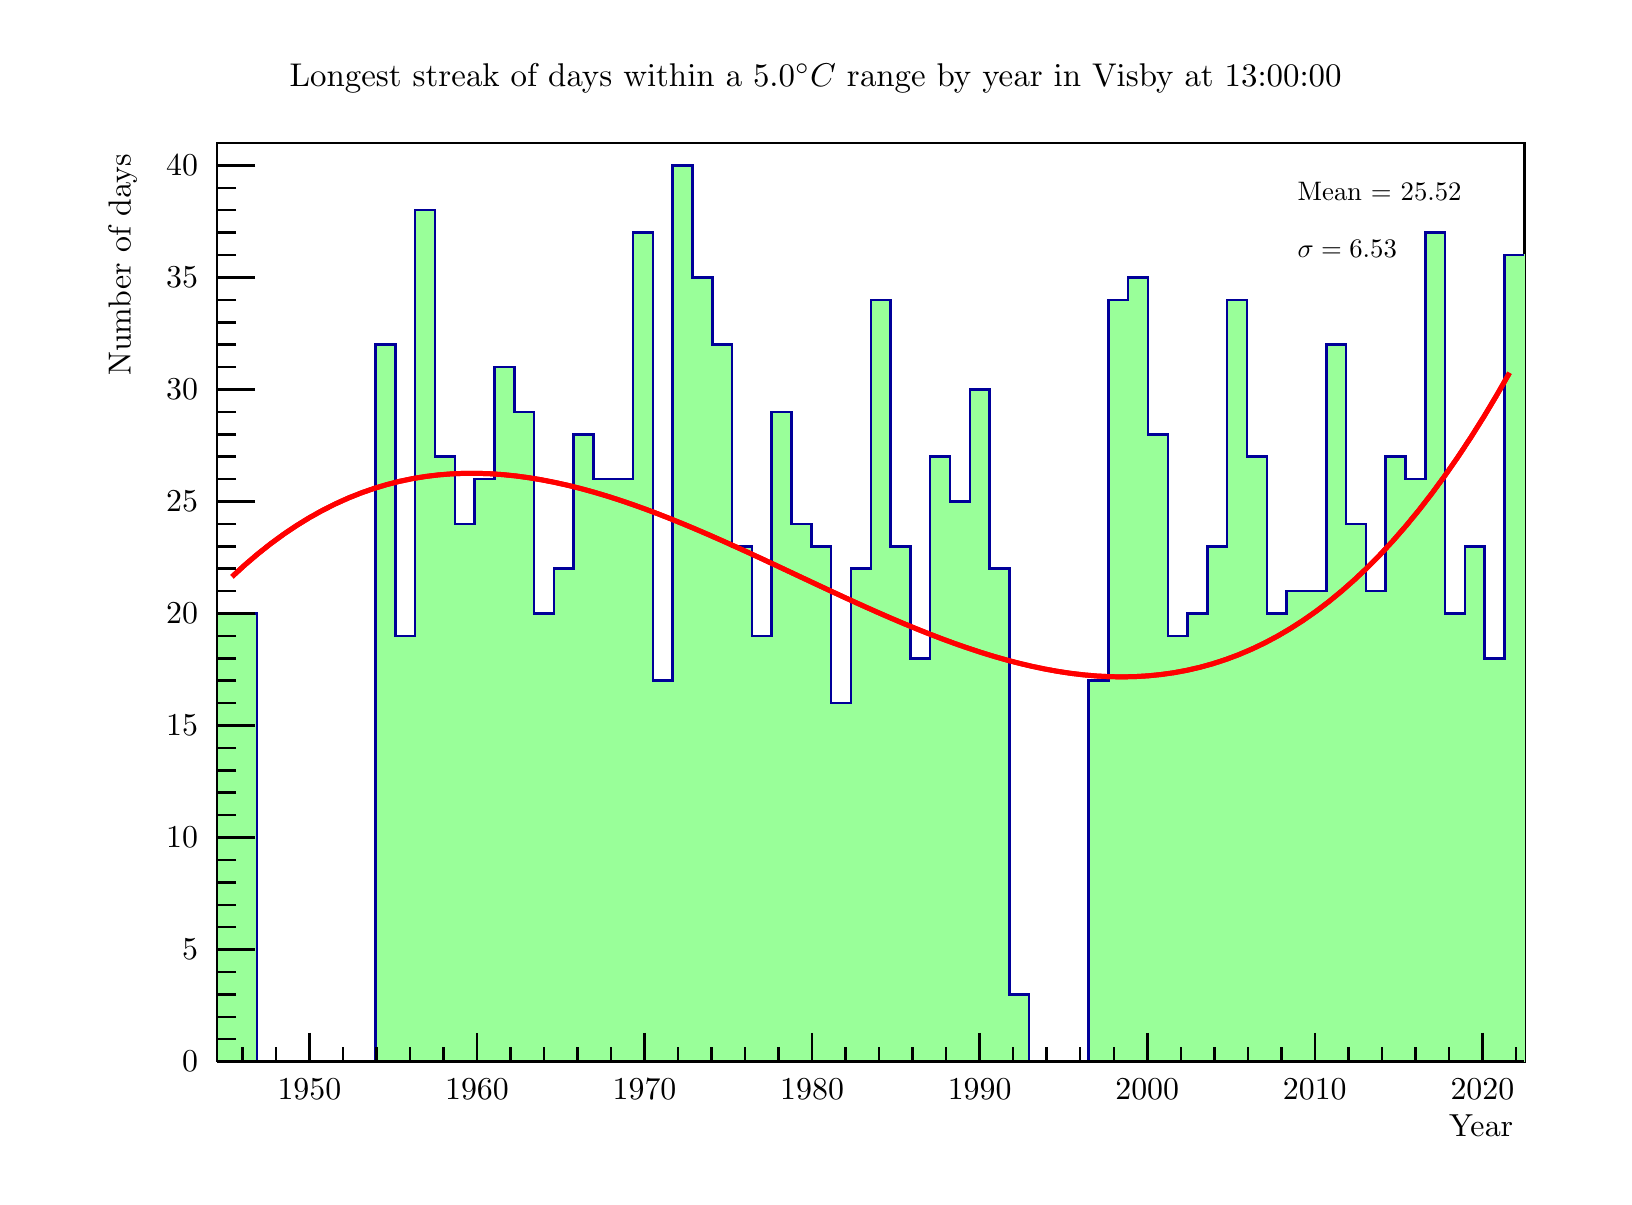
\begin{tikzpicture}
\def\CheckTikzLibraryLoaded#1{ \ifcsname tikz@library@#1@loaded\endcsname \else \PackageWarning{tikz}{usetikzlibrary{#1} is missing in the preamble.} \fi }
\CheckTikzLibraryLoaded{patterns}
\CheckTikzLibraryLoaded{plotmarks}
\pgfdeclareplotmark{cross} {
\pgfpathmoveto{\pgfpoint{-0.3\pgfplotmarksize}{\pgfplotmarksize}}
\pgfpathlineto{\pgfpoint{+0.3\pgfplotmarksize}{\pgfplotmarksize}}
\pgfpathlineto{\pgfpoint{+0.3\pgfplotmarksize}{0.3\pgfplotmarksize}}
\pgfpathlineto{\pgfpoint{+1\pgfplotmarksize}{0.3\pgfplotmarksize}}
\pgfpathlineto{\pgfpoint{+1\pgfplotmarksize}{-0.3\pgfplotmarksize}}
\pgfpathlineto{\pgfpoint{+0.3\pgfplotmarksize}{-0.3\pgfplotmarksize}}
\pgfpathlineto{\pgfpoint{+0.3\pgfplotmarksize}{-1.\pgfplotmarksize}}
\pgfpathlineto{\pgfpoint{-0.3\pgfplotmarksize}{-1.\pgfplotmarksize}}
\pgfpathlineto{\pgfpoint{-0.3\pgfplotmarksize}{-0.3\pgfplotmarksize}}
\pgfpathlineto{\pgfpoint{-1.\pgfplotmarksize}{-0.3\pgfplotmarksize}}
\pgfpathlineto{\pgfpoint{-1.\pgfplotmarksize}{0.3\pgfplotmarksize}}
\pgfpathlineto{\pgfpoint{-0.3\pgfplotmarksize}{0.3\pgfplotmarksize}}
\pgfpathclose
\pgfusepathqstroke
}
\pgfdeclareplotmark{cross*} {
\pgfpathmoveto{\pgfpoint{-0.3\pgfplotmarksize}{\pgfplotmarksize}}
\pgfpathlineto{\pgfpoint{+0.3\pgfplotmarksize}{\pgfplotmarksize}}
\pgfpathlineto{\pgfpoint{+0.3\pgfplotmarksize}{0.3\pgfplotmarksize}}
\pgfpathlineto{\pgfpoint{+1\pgfplotmarksize}{0.3\pgfplotmarksize}}
\pgfpathlineto{\pgfpoint{+1\pgfplotmarksize}{-0.3\pgfplotmarksize}}
\pgfpathlineto{\pgfpoint{+0.3\pgfplotmarksize}{-0.3\pgfplotmarksize}}
\pgfpathlineto{\pgfpoint{+0.3\pgfplotmarksize}{-1.\pgfplotmarksize}}
\pgfpathlineto{\pgfpoint{-0.3\pgfplotmarksize}{-1.\pgfplotmarksize}}
\pgfpathlineto{\pgfpoint{-0.3\pgfplotmarksize}{-0.3\pgfplotmarksize}}
\pgfpathlineto{\pgfpoint{-1.\pgfplotmarksize}{-0.3\pgfplotmarksize}}
\pgfpathlineto{\pgfpoint{-1.\pgfplotmarksize}{0.3\pgfplotmarksize}}
\pgfpathlineto{\pgfpoint{-0.3\pgfplotmarksize}{0.3\pgfplotmarksize}}
\pgfpathclose
\pgfusepathqfillstroke
}
\pgfdeclareplotmark{newstar} {
\pgfpathmoveto{\pgfqpoint{0pt}{\pgfplotmarksize}}
\pgfpathlineto{\pgfqpointpolar{44}{0.5\pgfplotmarksize}}
\pgfpathlineto{\pgfqpointpolar{18}{\pgfplotmarksize}}
\pgfpathlineto{\pgfqpointpolar{-20}{0.5\pgfplotmarksize}}
\pgfpathlineto{\pgfqpointpolar{-54}{\pgfplotmarksize}}
\pgfpathlineto{\pgfqpointpolar{-90}{0.5\pgfplotmarksize}}
\pgfpathlineto{\pgfqpointpolar{234}{\pgfplotmarksize}}
\pgfpathlineto{\pgfqpointpolar{198}{0.5\pgfplotmarksize}}
\pgfpathlineto{\pgfqpointpolar{162}{\pgfplotmarksize}}
\pgfpathlineto{\pgfqpointpolar{134}{0.5\pgfplotmarksize}}
\pgfpathclose
\pgfusepathqstroke
}
\pgfdeclareplotmark{newstar*} {
\pgfpathmoveto{\pgfqpoint{0pt}{\pgfplotmarksize}}
\pgfpathlineto{\pgfqpointpolar{44}{0.5\pgfplotmarksize}}
\pgfpathlineto{\pgfqpointpolar{18}{\pgfplotmarksize}}
\pgfpathlineto{\pgfqpointpolar{-20}{0.5\pgfplotmarksize}}
\pgfpathlineto{\pgfqpointpolar{-54}{\pgfplotmarksize}}
\pgfpathlineto{\pgfqpointpolar{-90}{0.5\pgfplotmarksize}}
\pgfpathlineto{\pgfqpointpolar{234}{\pgfplotmarksize}}
\pgfpathlineto{\pgfqpointpolar{198}{0.5\pgfplotmarksize}}
\pgfpathlineto{\pgfqpointpolar{162}{\pgfplotmarksize}}
\pgfpathlineto{\pgfqpointpolar{134}{0.5\pgfplotmarksize}}
\pgfpathclose
\pgfusepathqfillstroke
}
\definecolor{c}{rgb}{1,1,1};
\draw [color=c, fill=c] (0,0) rectangle (20,14.5819);
\draw [color=c, fill=c] (2.4,1.45819) rectangle (19,13.1237);
\definecolor{c}{rgb}{0,0,0};
\draw [c,line width=0.9] (2.4,1.45819) -- (2.4,13.1237) -- (19,13.1237) -- (19,1.45819) -- (2.4,1.45819);
\definecolor{c}{rgb}{1,1,1};
\draw [color=c, fill=c] (2.4,1.45819) rectangle (19,13.1237);
\definecolor{c}{rgb}{0,0,0};
\draw [c,line width=0.9] (2.4,1.45819) -- (2.4,13.1237) -- (19,13.1237) -- (19,1.45819) -- (2.4,1.45819);
\definecolor{c}{rgb}{0.6,1,0.6};
\draw [c, fill=c] (2.4,1.45819) -- (2.4,7.14871) -- (2.65152,7.14871) -- (2.65152,7.14871) -- (2.90303,7.14871) -- (2.90303,1.45819) -- (3.15455,1.45819) -- (3.15455,1.45819) -- (3.40606,1.45819) -- (3.40606,1.45819) -- (3.65758,1.45819) --
 (3.65758,1.45819) -- (3.90909,1.45819) -- (3.90909,1.45819) -- (4.16061,1.45819) -- (4.16061,1.45819) -- (4.41212,1.45819) -- (4.41212,10.563) -- (4.66364,10.563) -- (4.66364,6.86418) -- (4.91515,6.86418) -- (4.91515,12.2702) -- (5.16667,12.2702) --
 (5.16667,9.14039) -- (5.41818,9.14039) -- (5.41818,8.28681) -- (5.6697,8.28681) -- (5.6697,8.85586) -- (5.92121,8.85586) -- (5.92121,10.2785) -- (6.17273,10.2785) -- (6.17273,9.70944) -- (6.42424,9.70944) -- (6.42424,7.14871) -- (6.67576,7.14871) --
 (6.67576,7.71776) -- (6.92727,7.71776) -- (6.92727,9.42491) -- (7.17879,9.42491) -- (7.17879,8.85586) -- (7.4303,8.85586) -- (7.4303,8.85586) -- (7.68182,8.85586) -- (7.68182,11.9856) -- (7.93333,11.9856) -- (7.93333,6.29513) -- (8.18485,6.29513) --
 (8.18485,12.8392) -- (8.43636,12.8392) -- (8.43636,11.4166) -- (8.68788,11.4166) -- (8.68788,10.563) -- (8.93939,10.563) -- (8.93939,8.00228) -- (9.19091,8.00228) -- (9.19091,6.86418) -- (9.44242,6.86418) -- (9.44242,9.70944) -- (9.69394,9.70944) --
 (9.69394,8.28681) -- (9.94545,8.28681) -- (9.94545,8.00228) -- (10.197,8.00228) -- (10.197,6.0106) -- (10.4485,6.0106) -- (10.4485,7.71776) -- (10.7,7.71776) -- (10.7,11.1321) -- (10.9515,11.1321) -- (10.9515,8.00228) -- (11.203,8.00228) --
 (11.203,6.57966) -- (11.4545,6.57966) -- (11.4545,9.14039) -- (11.7061,9.14039) -- (11.7061,8.57133) -- (11.9576,8.57133) -- (11.9576,9.99396) -- (12.2091,9.99396) -- (12.2091,7.71776) -- (12.4606,7.71776) -- (12.4606,2.31177) -- (12.7121,2.31177)
 -- (12.7121,1.45819) -- (12.9636,1.45819) -- (12.9636,1.45819) -- (13.2152,1.45819) -- (13.2152,1.45819) -- (13.4667,1.45819) -- (13.4667,6.29513) -- (13.7182,6.29513) -- (13.7182,11.1321) -- (13.9697,11.1321) -- (13.9697,11.4166) --
 (14.2212,11.4166) -- (14.2212,9.42491) -- (14.4727,9.42491) -- (14.4727,6.86418) -- (14.7242,6.86418) -- (14.7242,7.14871) -- (14.9758,7.14871) -- (14.9758,8.00228) -- (15.2273,8.00228) -- (15.2273,11.1321) -- (15.4788,11.1321) -- (15.4788,9.14039)
 -- (15.7303,9.14039) -- (15.7303,7.14871) -- (15.9818,7.14871) -- (15.9818,7.43323) -- (16.2333,7.43323) -- (16.2333,7.43323) -- (16.4848,7.43323) -- (16.4848,10.563) -- (16.7364,10.563) -- (16.7364,8.28681) -- (16.9879,8.28681) -- (16.9879,7.43323)
 -- (17.2394,7.43323) -- (17.2394,9.14039) -- (17.4909,9.14039) -- (17.4909,8.85586) -- (17.7424,8.85586) -- (17.7424,11.9856) -- (17.9939,11.9856) -- (17.9939,7.14871) -- (18.2455,7.14871) -- (18.2455,8.00228) -- (18.497,8.00228) -- (18.497,6.57966)
 -- (18.7485,6.57966) -- (18.7485,11.7011) -- (19,11.7011) -- (19,1.45819);
\definecolor{c}{rgb}{0,0,0.6};
\draw [c,line width=0.9] (2.4,7.14871) -- (2.65152,7.14871) -- (2.65152,7.14871) -- (2.90303,7.14871) -- (2.90303,1.45819) -- (3.15455,1.45819) -- (3.15455,1.45819) -- (3.40606,1.45819) -- (3.40606,1.45819) -- (3.65758,1.45819) -- (3.65758,1.45819)
 -- (3.90909,1.45819) -- (3.90909,1.45819) -- (4.16061,1.45819) -- (4.16061,1.45819) -- (4.41212,1.45819) -- (4.41212,10.563) -- (4.66364,10.563) -- (4.66364,6.86418) -- (4.91515,6.86418) -- (4.91515,12.2702) -- (5.16667,12.2702) -- (5.16667,9.14039)
 -- (5.41818,9.14039) -- (5.41818,8.28681) -- (5.6697,8.28681) -- (5.6697,8.85586) -- (5.92121,8.85586) -- (5.92121,10.2785) -- (6.17273,10.2785) -- (6.17273,9.70944) -- (6.42424,9.70944) -- (6.42424,7.14871) -- (6.67576,7.14871) -- (6.67576,7.71776)
 -- (6.92727,7.71776) -- (6.92727,9.42491) -- (7.17879,9.42491) -- (7.17879,8.85586) -- (7.4303,8.85586) -- (7.4303,8.85586) -- (7.68182,8.85586) -- (7.68182,11.9856) -- (7.93333,11.9856) -- (7.93333,6.29513) -- (8.18485,6.29513) -- (8.18485,12.8392)
 -- (8.43636,12.8392) -- (8.43636,11.4166) -- (8.68788,11.4166) -- (8.68788,10.563) -- (8.93939,10.563) -- (8.93939,8.00228) -- (9.19091,8.00228) -- (9.19091,6.86418) -- (9.44242,6.86418) -- (9.44242,9.70944) -- (9.69394,9.70944) -- (9.69394,8.28681)
 -- (9.94545,8.28681) -- (9.94545,8.00228) -- (10.197,8.00228) -- (10.197,6.0106) -- (10.4485,6.0106) -- (10.4485,7.71776) -- (10.7,7.71776) -- (10.7,11.1321) -- (10.9515,11.1321) -- (10.9515,8.00228) -- (11.203,8.00228) -- (11.203,6.57966) --
 (11.4545,6.57966) -- (11.4545,9.14039) -- (11.7061,9.14039) -- (11.7061,8.57133) -- (11.9576,8.57133) -- (11.9576,9.99396) -- (12.2091,9.99396) -- (12.2091,7.71776) -- (12.4606,7.71776) -- (12.4606,2.31177) -- (12.7121,2.31177) -- (12.7121,1.45819)
 -- (12.9636,1.45819) -- (12.9636,1.45819) -- (13.2152,1.45819) -- (13.2152,1.45819) -- (13.4667,1.45819) -- (13.4667,6.29513) -- (13.7182,6.29513) -- (13.7182,11.1321) -- (13.9697,11.1321) -- (13.9697,11.4166) -- (14.2212,11.4166) --
 (14.2212,9.42491) -- (14.4727,9.42491) -- (14.4727,6.86418) -- (14.7242,6.86418) -- (14.7242,7.14871) -- (14.9758,7.14871) -- (14.9758,8.00228) -- (15.2273,8.00228) -- (15.2273,11.1321) -- (15.4788,11.1321) -- (15.4788,9.14039) -- (15.7303,9.14039)
 -- (15.7303,7.14871) -- (15.9818,7.14871) -- (15.9818,7.43323) -- (16.2333,7.43323) -- (16.2333,7.43323) -- (16.4848,7.43323) -- (16.4848,10.563) -- (16.7364,10.563) -- (16.7364,8.28681) -- (16.9879,8.28681) -- (16.9879,7.43323) -- (17.2394,7.43323)
 -- (17.2394,9.14039) -- (17.4909,9.14039) -- (17.4909,8.85586) -- (17.7424,8.85586) -- (17.7424,11.9856) -- (17.9939,11.9856) -- (17.9939,7.14871) -- (18.2455,7.14871) -- (18.2455,8.00228) -- (18.497,8.00228) -- (18.497,6.57966) -- (18.7485,6.57966)
 -- (18.7485,11.7011) -- (19,11.7011);
\definecolor{c}{rgb}{1,0,0};
\draw [c,line width=1.8] (2.58835,7.61614) -- (2.75222,7.7663) -- (2.91609,7.90608) -- (3.07996,8.03572) -- (3.24383,8.15546) -- (3.40771,8.26555) -- (3.57158,8.36623) -- (3.73545,8.45775) -- (3.89932,8.54034) -- (4.06319,8.61425) --
 (4.22706,8.67972) -- (4.39094,8.73699) -- (4.55481,8.78632) -- (4.71868,8.82793) -- (4.88255,8.86207) -- (5.04642,8.88899) -- (5.21029,8.90893) -- (5.37417,8.92213) -- (5.53804,8.92883) -- (5.70191,8.92928) -- (5.86578,8.92371) -- (6.02965,8.91238)
 -- (6.19353,8.89553) -- (6.3574,8.87339) -- (6.52127,8.84621) -- (6.68514,8.81424) -- (6.84901,8.77771) -- (7.01288,8.73687) -- (7.17676,8.69196) -- (7.34063,8.64323) -- (7.5045,8.59091) -- (7.66837,8.53525) -- (7.83224,8.4765) -- (7.99612,8.41489)
 -- (8.15999,8.35067) -- (8.32386,8.28408) -- (8.48773,8.21536) -- (8.6516,8.14476) -- (8.81547,8.07252) -- (8.97935,7.99888) -- (9.14322,7.92409) -- (9.30709,7.84839) -- (9.47096,7.77201) -- (9.63483,7.69521) -- (9.79871,7.61823) -- (9.96258,7.5413)
 -- (10.1264,7.46467) -- (10.2903,7.38859) -- (10.4542,7.3133) -- (10.6181,7.23904);
\draw [c,line width=1.8] (10.6181,7.23904) -- (10.7819,7.16605) -- (10.9458,7.09458) -- (11.1097,7.02486) -- (11.2736,6.95715) -- (11.4374,6.89167) -- (11.6013,6.82869) -- (11.7652,6.76844) -- (11.929,6.71116) -- (12.0929,6.65709) --
 (12.2568,6.60648) -- (12.4207,6.55957) -- (12.5845,6.51661) -- (12.7484,6.47783) -- (12.9123,6.44348) -- (13.0761,6.4138) -- (13.24,6.38904) -- (13.4039,6.36944) -- (13.5678,6.35523) -- (13.7316,6.34667) -- (13.8955,6.34399) -- (14.0594,6.34745) --
 (14.2232,6.35727) -- (14.3871,6.37371) -- (14.551,6.397) -- (14.7149,6.4274) -- (14.8787,6.46514) -- (15.0426,6.51046) -- (15.2065,6.56361) -- (15.3703,6.62483) -- (15.5342,6.69437) -- (15.6981,6.77246) -- (15.862,6.85935) -- (16.0258,6.95528) --
 (16.1897,7.0605) -- (16.3536,7.17525) -- (16.5174,7.29976) -- (16.6813,7.43429) -- (16.8452,7.57908) -- (17.0091,7.73436) -- (17.1729,7.90039) -- (17.3368,8.0774) -- (17.5007,8.26564) -- (17.6646,8.46534) -- (17.8284,8.67676) -- (17.9923,8.90014) --
 (18.1562,9.13571) -- (18.32,9.38373) -- (18.4839,9.64443) -- (18.6478,9.91805);
\draw [c,line width=1.8] (18.6478,9.91805) -- (18.8117,10.2048);
\definecolor{c}{rgb}{0,0,0};
\draw [c,line width=0.9] (2.4,1.45819) -- (19,1.45819);
\draw [c,line width=0.9] (3.57051,1.82128) -- (3.57051,1.45819);
\draw [c,line width=0.9] (3.99615,1.63974) -- (3.99615,1.45819);
\draw [c,line width=0.9] (4.42179,1.63974) -- (4.42179,1.45819);
\draw [c,line width=0.9] (4.84744,1.63974) -- (4.84744,1.45819);
\draw [c,line width=0.9] (5.27308,1.63974) -- (5.27308,1.45819);
\draw [c,line width=0.9] (5.69872,1.82128) -- (5.69872,1.45819);
\draw [c,line width=0.9] (6.12436,1.63974) -- (6.12436,1.45819);
\draw [c,line width=0.9] (6.55,1.63974) -- (6.55,1.45819);
\draw [c,line width=0.9] (6.97564,1.63974) -- (6.97564,1.45819);
\draw [c,line width=0.9] (7.40128,1.63974) -- (7.40128,1.45819);
\draw [c,line width=0.9] (7.82692,1.82128) -- (7.82692,1.45819);
\draw [c,line width=0.9] (8.25256,1.63974) -- (8.25256,1.45819);
\draw [c,line width=0.9] (8.67821,1.63974) -- (8.67821,1.45819);
\draw [c,line width=0.9] (9.10385,1.63974) -- (9.10385,1.45819);
\draw [c,line width=0.9] (9.52949,1.63974) -- (9.52949,1.45819);
\draw [c,line width=0.9] (9.95513,1.82128) -- (9.95513,1.45819);
\draw [c,line width=0.9] (10.3808,1.63974) -- (10.3808,1.45819);
\draw [c,line width=0.9] (10.8064,1.63974) -- (10.8064,1.45819);
\draw [c,line width=0.9] (11.2321,1.63974) -- (11.2321,1.45819);
\draw [c,line width=0.9] (11.6577,1.63974) -- (11.6577,1.45819);
\draw [c,line width=0.9] (12.0833,1.82128) -- (12.0833,1.45819);
\draw [c,line width=0.9] (12.509,1.63974) -- (12.509,1.45819);
\draw [c,line width=0.9] (12.9346,1.63974) -- (12.9346,1.45819);
\draw [c,line width=0.9] (13.3603,1.63974) -- (13.3603,1.45819);
\draw [c,line width=0.9] (13.7859,1.63974) -- (13.7859,1.45819);
\draw [c,line width=0.9] (14.2115,1.82128) -- (14.2115,1.45819);
\draw [c,line width=0.9] (14.6372,1.63974) -- (14.6372,1.45819);
\draw [c,line width=0.9] (15.0628,1.63974) -- (15.0628,1.45819);
\draw [c,line width=0.9] (15.4885,1.63974) -- (15.4885,1.45819);
\draw [c,line width=0.9] (15.9141,1.63974) -- (15.9141,1.45819);
\draw [c,line width=0.9] (16.3397,1.82128) -- (16.3397,1.45819);
\draw [c,line width=0.9] (16.7654,1.63974) -- (16.7654,1.45819);
\draw [c,line width=0.9] (17.191,1.63974) -- (17.191,1.45819);
\draw [c,line width=0.9] (17.6167,1.63974) -- (17.6167,1.45819);
\draw [c,line width=0.9] (18.0423,1.63974) -- (18.0423,1.45819);
\draw [c,line width=0.9] (18.4679,1.82128) -- (18.4679,1.45819);
\draw [c,line width=0.9] (3.57051,1.82128) -- (3.57051,1.45819);
\draw [c,line width=0.9] (3.14487,1.63974) -- (3.14487,1.45819);
\draw [c,line width=0.9] (2.71923,1.63974) -- (2.71923,1.45819);
\draw [c,line width=0.9] (18.4679,1.82128) -- (18.4679,1.45819);
\draw [c,line width=0.9] (18.8936,1.63974) -- (18.8936,1.45819);
\draw [anchor=base] (3.57051,0.97699) node[scale=1.15134, color=c, rotate=0]{1950};
\draw [anchor=base] (5.69872,0.97699) node[scale=1.15134, color=c, rotate=0]{1960};
\draw [anchor=base] (7.82692,0.97699) node[scale=1.15134, color=c, rotate=0]{1970};
\draw [anchor=base] (9.95513,0.97699) node[scale=1.15134, color=c, rotate=0]{1980};
\draw [anchor=base] (12.0833,0.97699) node[scale=1.15134, color=c, rotate=0]{1990};
\draw [anchor=base] (14.2115,0.97699) node[scale=1.15134, color=c, rotate=0]{2000};
\draw [anchor=base] (16.3397,0.97699) node[scale=1.15134, color=c, rotate=0]{2010};
\draw [anchor=base] (18.4679,0.97699) node[scale=1.15134, color=c, rotate=0]{2020};
\draw [anchor= east] (19,0.641605) node[scale=1.15134, color=c, rotate=0]{Year};
\draw [c,line width=0.9] (2.4,1.45819) -- (2.4,13.1237);
\draw [c,line width=0.9] (2.88,1.45819) -- (2.4,1.45819);
\draw [c,line width=0.9] (2.64,1.74272) -- (2.4,1.74272);
\draw [c,line width=0.9] (2.64,2.02725) -- (2.4,2.02725);
\draw [c,line width=0.9] (2.64,2.31177) -- (2.4,2.31177);
\draw [c,line width=0.9] (2.64,2.5963) -- (2.4,2.5963);
\draw [c,line width=0.9] (2.88,2.88082) -- (2.4,2.88082);
\draw [c,line width=0.9] (2.64,3.16535) -- (2.4,3.16535);
\draw [c,line width=0.9] (2.64,3.44987) -- (2.4,3.44987);
\draw [c,line width=0.9] (2.64,3.7344) -- (2.4,3.7344);
\draw [c,line width=0.9] (2.64,4.01892) -- (2.4,4.01892);
\draw [c,line width=0.9] (2.88,4.30345) -- (2.4,4.30345);
\draw [c,line width=0.9] (2.64,4.58798) -- (2.4,4.58798);
\draw [c,line width=0.9] (2.64,4.8725) -- (2.4,4.8725);
\draw [c,line width=0.9] (2.64,5.15703) -- (2.4,5.15703);
\draw [c,line width=0.9] (2.64,5.44155) -- (2.4,5.44155);
\draw [c,line width=0.9] (2.88,5.72608) -- (2.4,5.72608);
\draw [c,line width=0.9] (2.64,6.0106) -- (2.4,6.0106);
\draw [c,line width=0.9] (2.64,6.29513) -- (2.4,6.29513);
\draw [c,line width=0.9] (2.64,6.57966) -- (2.4,6.57966);
\draw [c,line width=0.9] (2.64,6.86418) -- (2.4,6.86418);
\draw [c,line width=0.9] (2.88,7.14871) -- (2.4,7.14871);
\draw [c,line width=0.9] (2.64,7.43323) -- (2.4,7.43323);
\draw [c,line width=0.9] (2.64,7.71776) -- (2.4,7.71776);
\draw [c,line width=0.9] (2.64,8.00228) -- (2.4,8.00228);
\draw [c,line width=0.9] (2.64,8.28681) -- (2.4,8.28681);
\draw [c,line width=0.9] (2.88,8.57133) -- (2.4,8.57133);
\draw [c,line width=0.9] (2.64,8.85586) -- (2.4,8.85586);
\draw [c,line width=0.9] (2.64,9.14039) -- (2.4,9.14039);
\draw [c,line width=0.9] (2.64,9.42491) -- (2.4,9.42491);
\draw [c,line width=0.9] (2.64,9.70944) -- (2.4,9.70944);
\draw [c,line width=0.9] (2.88,9.99396) -- (2.4,9.99396);
\draw [c,line width=0.9] (2.64,10.2785) -- (2.4,10.2785);
\draw [c,line width=0.9] (2.64,10.563) -- (2.4,10.563);
\draw [c,line width=0.9] (2.64,10.8475) -- (2.4,10.8475);
\draw [c,line width=0.9] (2.64,11.1321) -- (2.4,11.1321);
\draw [c,line width=0.9] (2.88,11.4166) -- (2.4,11.4166);
\draw [c,line width=0.9] (2.64,11.7011) -- (2.4,11.7011);
\draw [c,line width=0.9] (2.64,11.9856) -- (2.4,11.9856);
\draw [c,line width=0.9] (2.64,12.2702) -- (2.4,12.2702);
\draw [c,line width=0.9] (2.64,12.5547) -- (2.4,12.5547);
\draw [c,line width=0.9] (2.88,12.8392) -- (2.4,12.8392);
\draw [c,line width=0.9] (2.88,12.8392) -- (2.4,12.8392);
\draw [anchor= east] (2.3,1.45819) node[scale=1.15134, color=c, rotate=0]{0};
\draw [anchor= east] (2.3,2.88082) node[scale=1.15134, color=c, rotate=0]{5};
\draw [anchor= east] (2.3,4.30345) node[scale=1.15134, color=c, rotate=0]{10};
\draw [anchor= east] (2.3,5.72608) node[scale=1.15134, color=c, rotate=0]{15};
\draw [anchor= east] (2.3,7.14871) node[scale=1.15134, color=c, rotate=0]{20};
\draw [anchor= east] (2.3,8.57133) node[scale=1.15134, color=c, rotate=0]{25};
\draw [anchor= east] (2.3,9.99396) node[scale=1.15134, color=c, rotate=0]{30};
\draw [anchor= east] (2.3,11.4166) node[scale=1.15134, color=c, rotate=0]{35};
\draw [anchor= east] (2.3,12.8392) node[scale=1.15134, color=c, rotate=0]{40};
\draw [anchor= east] (1.19833,13.1237) node[scale=1.15134, color=c, rotate=90]{Number of days};
\definecolor{c}{rgb}{1,0,0};
\draw [c,line width=1.8] (2.58835,7.61614) -- (2.75222,7.7663) -- (2.91609,7.90608) -- (3.07996,8.03572) -- (3.24383,8.15546) -- (3.40771,8.26555) -- (3.57158,8.36623) -- (3.73545,8.45775) -- (3.89932,8.54034) -- (4.06319,8.61425) --
 (4.22706,8.67972) -- (4.39094,8.73699) -- (4.55481,8.78632) -- (4.71868,8.82793) -- (4.88255,8.86207) -- (5.04642,8.88899) -- (5.21029,8.90893) -- (5.37417,8.92213) -- (5.53804,8.92883) -- (5.70191,8.92928) -- (5.86578,8.92371) -- (6.02965,8.91238)
 -- (6.19353,8.89553) -- (6.3574,8.87339) -- (6.52127,8.84621) -- (6.68514,8.81424) -- (6.84901,8.77771) -- (7.01288,8.73687) -- (7.17676,8.69196) -- (7.34063,8.64323) -- (7.5045,8.59091) -- (7.66837,8.53525) -- (7.83224,8.4765) -- (7.99612,8.41489)
 -- (8.15999,8.35067) -- (8.32386,8.28408) -- (8.48773,8.21536) -- (8.6516,8.14476) -- (8.81547,8.07252) -- (8.97935,7.99888) -- (9.14322,7.92409) -- (9.30709,7.84839) -- (9.47096,7.77201) -- (9.63483,7.69521) -- (9.79871,7.61823) -- (9.96258,7.5413)
 -- (10.1264,7.46467) -- (10.2903,7.38859) -- (10.4542,7.3133) -- (10.6181,7.23904);
\draw [c,line width=1.8] (10.6181,7.23904) -- (10.7819,7.16605) -- (10.9458,7.09458) -- (11.1097,7.02486) -- (11.2736,6.95715) -- (11.4374,6.89167) -- (11.6013,6.82869) -- (11.7652,6.76844) -- (11.929,6.71116) -- (12.0929,6.65709) --
 (12.2568,6.60648) -- (12.4207,6.55957) -- (12.5845,6.51661) -- (12.7484,6.47783) -- (12.9123,6.44348) -- (13.0761,6.4138) -- (13.24,6.38904) -- (13.4039,6.36944) -- (13.5678,6.35523) -- (13.7316,6.34667) -- (13.8955,6.34399) -- (14.0594,6.34745) --
 (14.2232,6.35727) -- (14.3871,6.37371) -- (14.551,6.397) -- (14.7149,6.4274) -- (14.8787,6.46514) -- (15.0426,6.51046) -- (15.2065,6.56361) -- (15.3703,6.62483) -- (15.5342,6.69437) -- (15.6981,6.77246) -- (15.862,6.85935) -- (16.0258,6.95528) --
 (16.1897,7.0605) -- (16.3536,7.17525) -- (16.5174,7.29976) -- (16.6813,7.43429) -- (16.8452,7.57908) -- (17.0091,7.73436) -- (17.1729,7.90039) -- (17.3368,8.0774) -- (17.5007,8.26564) -- (17.6646,8.46534) -- (17.8284,8.67676) -- (17.9923,8.90014) --
 (18.1562,9.13571) -- (18.32,9.38373) -- (18.4839,9.64443) -- (18.6478,9.91805);
\draw [c,line width=1.8] (18.6478,9.91805) -- (18.8117,10.2048);
\definecolor{c}{rgb}{0,0,0};
\draw [anchor=base west] (16,12.3946) node[scale=0.965639, color=c, rotate=0]{Mean = 25.52};
\draw [anchor=base west] (16,11.6656) node[scale=0.965639, color=c, rotate=0]{$\sigma = 6.53$};
\draw (10,13.9476) node[scale=1.18848, color=c, rotate=0]{$\text{Longest streak of days within a }5.0^{\circ}C\text{ range by year in }\text{Visby at 13:00:00}$};
\end{tikzpicture}}
    \label{fig:enter-label}
\end{figure}

\section{Conclusion}

The project's goals were achieved: the annual temperature data was analyzed by generating histograms that depict the count of days, streaks and amplitude variations within a given range.

The created histograms revealed interesting patterns, such as notable streaks and outliers.

\subsection{Possible Improvements}

The main possible improvement is that an output text file could be provided, describing specifically when long streaks or other points of interest occur. As it stands, there is no way of knowing on which days these happen without scouring through the CSV files manually.

\end{document}
    